\chapter{Fundamentos teóricos}
\label{c:parte3}
\vspace{1cm}
En este capítulo, se presentan los fundamentos teóricos sobre los cuales se sustenta el proyecto y particularmente el método luego utilizado. Primeramente se describen algunas operaciones morfológicas sobre imágenes y algunas técnicas de realce sobre las mismas. Tras ello, se explica un método de detección y descripción de características en imágenes. También, se presenta una técnica para búsqueda de correspondencias entre puntos característicos de imágenes, que sirve como base para encontrar la relación entre dos imágenes de un mismo objeto fotografiado desde diferentes perspectivas.
\section{Operaciones morfológicas en imágenes}
El procesamiento morfológico en imágenes es un tipo de procesamiento en el cual la forma espacial o estructura de los objetos en la imagen es modificada. La erosión y dilatación son dos operaciones morfológicas fundamentales que pueden ser aplicadas a imágenes en escala de grises o imágenes binarias. En esta sección se describen tanto la erosión como la dilatación enfocándose en imágenes binarias que son las utilizadas en este trabajo.

El lenguaje de la morfología matemática es el de la teoría de conjuntos y la misma representa objetos en las imágenes. Por ejemplo, el conjunto de todos los píxeles negros en una imagen binaria es una descripción morfológica completa de la imagen. En imágenes binarias, el conjunto en cuestión es miembro de un espacio entero 2-D $Z^2$, donde cada elemento del conjunto es una tupla (vector 2-D) cuyas coordenadas son las coordenadas $(x,y)$ de un píxel negro (o blanco, dependiendo de la convención) de la imagen.

A continuación, definiremos algunas notaciones que serán utilizadas para definir posteriormente la erosión y la dilatación: nos referiremos con $A$ a un conjunto en $Z^2$, $a=(a_1,a_2)$ un elemento de $A$, $\varnothing$ un conjunto vacío, $A \subseteq B$ para denotar que $A$ es un subconjunto de $B$,  $A \cap B$ para indicar la intersección entre $A$ y $B$ (el conjunto de elementos que corresponde tanto a $A$ como a $B$), $\hat{B}=\{w|w=-b, \; \textrm{para} \; b \in B\}$ para indicar la reflexión del conjunto $B$,  $(A)_{z}=\{c|c=a+z,\; \textrm{para}\; a \in A\}$ para indicar la traslación del conjunto $A$ por $z=(z_1, z_2)$ y $\{\cdot\}$ la notación de un conjunto.
\subsection{Dilatación}
Sea $A$ y $B$ un conjunto en $Z^2$, la dilatación entre $A$ y $B$ denotada como $A \oplus B$ queda definida como
\begin{equation}
A\oplus B=\{z|(\hat{B})_{z}\cap\; A \neq \varnothing\},
\label{eq:eq_dilatacion}
\end{equation}
%De la expresión \ref{eq:eq_dilatacion}, se puede decir que la dilatación se basa en obtener la reflexión de $B$ sobre su origen y tras ello hace una traslación por $z$. 
donde $B$ comúnmente es conocido como máscara o kernel.

Mediante la dilatación, los objetos crecen en su tamaño y algunos de los ``espacios'' dentro de ellos son rellenados. Un ejemplo de dilatación sobre la imagen de la Fig. \ref{fig:original_erode_dilate} utilizando el kernel de la Fig. \ref{fig:mascara}, se puede observar en la Fig. \ref{fig:dilatacion_example} (se realizaron 2 dilataciones para resaltar el efecto de la operación).
% \begin{figure}[tbhp]
%    \centering
%         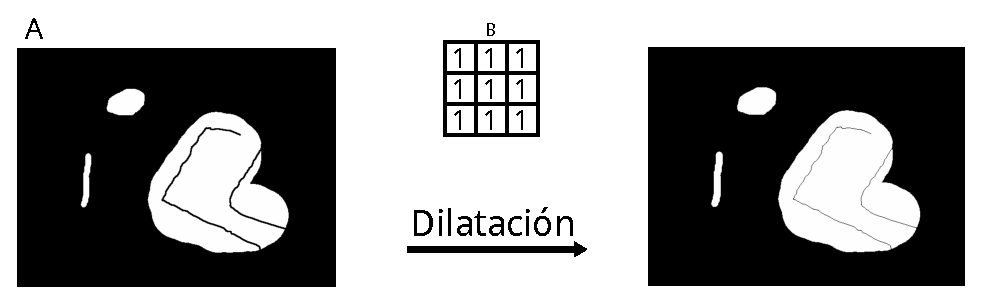
\includegraphics[scale=0.75]{../figs/dilatacion_example}
%      \caption[Dilatación de una imagen]{}
%    \label{}                %% Etiqueta para la figura entera
% \end{figure}
\subsection{Erosión}
Sea un conjunto $A$ y $B$ de $Z^2$, la erosión de $A$ por $B$, denotada como $A \ominus B$ queda definida como
\begin{equation}
A \ominus B=\{z|(B)_{z} \subseteq A\}.
\label{eq:eq_erosion}
\end{equation}
De la ecuación \eqref{eq:eq_erosion} se puede interpretar que la erosión de $A$ por $B$ es el conjunto de todos los puntos $z$ tales que $B$, trasladados por $z$, están contenidos en $A$.

Uno de los usos más simples de la erosión es la eliminación de detalles irrelevantes (en términos de tamaño) de una imagen binaria. En una imagen erosionada, el tamaño de los objetos se ve reducido y el ruido o detalles irrelevantes (aislados) es eliminado. Un ejemplo de erosión sobre la imagen de la Fig. \ref{fig:original_erode_dilate} utilizando el kernel de la Fig. \ref{fig:mascara}, se puede observar en la Fig. \ref{fig:erosion_example} (se realizaron 2 erosiones para resaltar el efecto de la operación).
% \begin{figure}[tbhp]
%    \centering
%         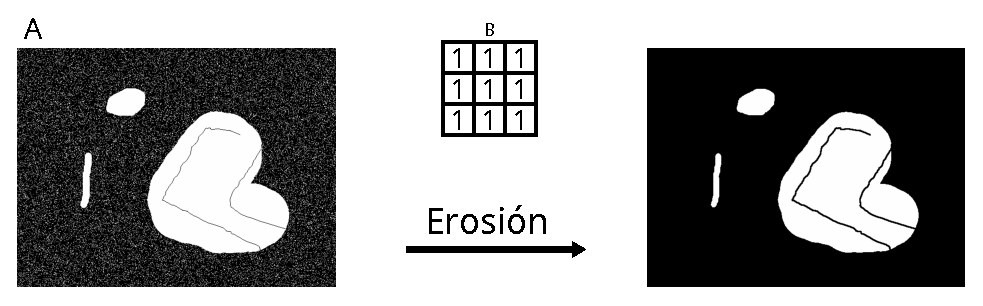
\includegraphics[scale=0.75]{../figs/erosion_example}
%     \caption[Erosión de una imagen]{Erosión de una imagen con una máscara (B) de $3\times3$.}
%    \label{fig:erosion_example}                %% Etiqueta para la figura entera
% \end{figure}
% % 
% Los filtros morfológicos son operadores que transforman una imagen de una forma predefinida (de acuerdo a la forma de la máscara aplicada). La interacción entre el filtro y los vecinos al píxel sobre el cuál se está aplicando el procesamiento, dan el resultado final de la transformación.
% 
% Técnicas como erosión, dilatación, entre otras, son algunas clases de este tipo de operaciones que poseen muchas aplicaciones y que en ocasiones son parte de un pre-procesamiento sobre las imágenes, para su posterior tratamiento con el objetivo de detectar una zona sobre la cual aplicar el procesamiento o eliminar zonas que resulten irrelevantes.
% 
% \subsection{Erosión y dilatación}
% Las erosión y dilatación son dos operaciones morfológicas usadas en variedad de contextos como remoción de ruido, aislación/unión de elementos, etc.
% 
% 
% 
% % Estos dos filtros operan sobre un conjunto de píxeles vecinos alrededor de cada píxel de la imagen sobre la cual es aplicada la operación.
% 
% La \emph{erosión}, reemplaza al píxel actual con el valor mínimo de la vecindad definida mediante un kernel, mientras que la \emph{dilatación} es la operación complementaria a la anterior, es decir, que reemplaza el píxel actual con el valor máximo del conjunto de píxeles vecinos definidos mediante el kernel. Así, en el caso de una imagen binaria (sólo contiene píxeles negros o blancos representados en nuestro caso con el valor 0 y 255), cada píxel es reemplazado por uno negro o blanco.  En el caso de la dilatación, los objetos crecen en su tamaño y algunos de los espacios dentro de ellos son rellenados.
% 
% % Una buena forma de ver el efecto de este operador es en términos de una imagen con fondo negro y objetos blancos. Cuando se aplica la erosión, si un píxel del filtro aplicado esta sobre el fondo, luego el píxel sobre el cuál se esta aplicando la erosión resultará con el valor del fondo. Mientras, que en el caso de la dilatación, si el filtro toca un objeto sobre el fodno, el pixel será asignado al valor del blanco. 
% % poner que máscara se usa y poner imagen
% % cvErode(frameDiferencia, frameDiferencia, NULL, 2);
% % cvDilate(frameDiferencia, frameDiferencia, NULL, 2);
% %http://opencv.willowgarage.com/documentation/miscellaneous_image_transformations.html?highlight=cvthreshold#cvThreshold
\begin{figure}[tbhp]
\centering
\subfloat[][Imagen sobre la que se realizan las operaciones (Figura tomada de \cite{Gonzalez:02}).]{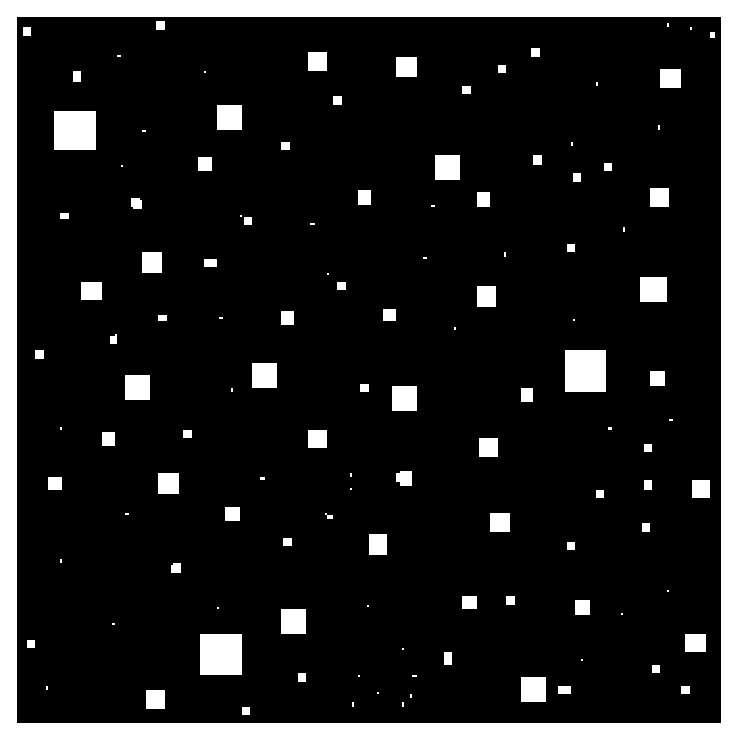
\includegraphics[width=2.3in]{../figs/erode_dilate/orig} \label{fig:original_erode_dilate}}  \qquad
\subfloat[][Kernel o máscara de $3\times3$.]{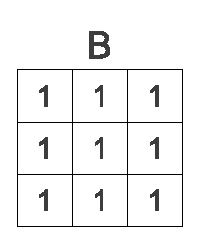
\includegraphics[width=1.0in]{../figs/mascara} \label{fig:mascara}}\\
\subfloat[][Dilatación ($\times$2).]{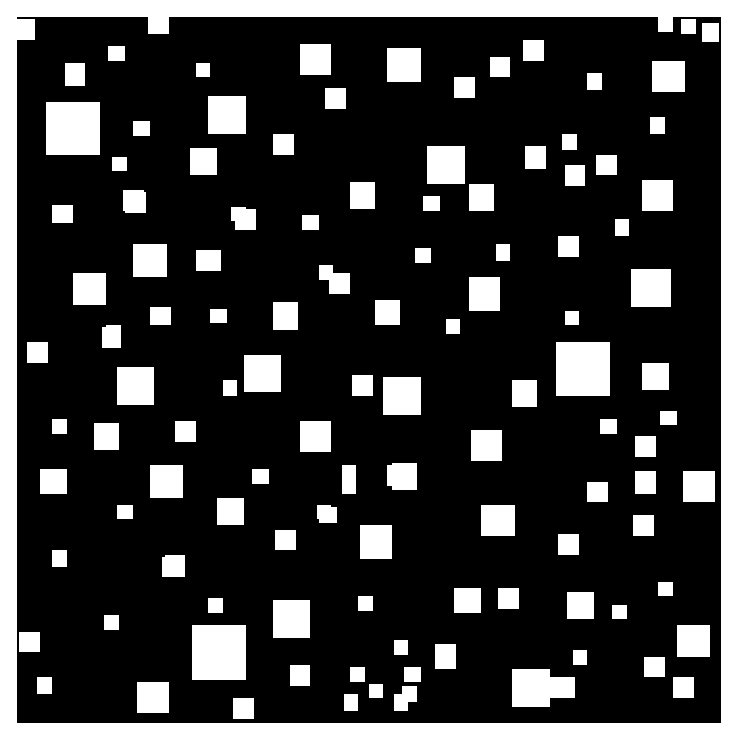
\includegraphics[width=2.3in]{../figs/erode_dilate/2dilate} \label{fig:dilatacion_example}}
\subfloat[][Erosión ($\times$2).]{\includegraphics[width=2.3in]{../figs/erode_dilate/2erode} \label{fig:erosion_example}}
\caption[Efecto de la operación de erosión y dilatación sobre una imagen]{Efecto de la operación de erosión y dilatación sobre la imagen \subref{fig:original_erode_dilate}. \subref{fig:mascara} Máscara o kernel utilizado para cada una de las operaciones. \subref{fig:dilatacion_example} Resultado de aplicar la dilatación ($\times2$). \subref{fig:erosion_example} Resultado de aplicar la erosión ($\times2$).
}
\end{figure}
\section{Realce de imágenes en el dominio espacial}
\label{subsec:mejoras_iluminacion}
En esta sección se presentan brevemente algunas técnicas en el dominio espacial. Las mismas, fueron seleccionadas debido a que presentan tiempos de cálculo pequeños y son orientadas a la tarea de realce de detalles o mejora de la iluminación en las imágenes.

Los métodos en el dominio espacial son procedimientos que operan directamente sobre los píxeles de la imagen y pueden denotase con la expresión $g(x,y)=T[f(x,y)]$, donde $f(x,y)$ es la imagen de entrada, $g(x,y)$ es la imagen resultado de la operación y $T$ es un operador sobre $f$ definido sobre alguna vecindad alrededor de $(x,y)$ \cite{Gonzalez:02}. 

El enfoque principal en la definición de la vecindad alrededor de un punto $(x,y)$, es el uso de una zona de sub imagen cuadrada o rectangular centrada en $(x,y)$. Cuando esta vecindad se establece a un valor de $1 \times 1$ (un píxel), $g$ depende únicamente del valor de $f$ en $(x,y)$ y $T$ se convierte en una función de transformación de intensidad de la forma $s=T(r)$. Dado que en este proyecto se trabaja con imágenes en escala de grises, $r$ y $s$ son variables que denotan el nivel de gris de $f(x,y)$ y $g(x,y)$ en el punto $(x,y)$ respectivamente.
\subsection{Umbral}
Podemos definir una función de umbral como una transformación con la forma de la expresión \eqref{eq:equation_umbral_binario} donde $r_{max}$ y $s_{max}$ son los valores máximos de intensidad de la imagen $f(x,y)$ y $g(x,y)$ respectivamente y $u$ una constante que define el valor de umbral de la transformación.

La función de umbral particular presentada en la Fig. \ref{fig:umbral_curve} produce una imagen binaria asignando el valor $s_{max}$ a los valores que superan $u$ y $0$ a los demás.
\begin{equation}
\label{eq:equation_umbral_binario}
s= 
\begin{cases} 0 & \text{para $r<u$,}
\\
s_{max} &\text{para $r>=u$}
\end{cases} \textrm{con } 0 \leq r \leq r_{max} \textrm{ y } 0 \leq u \leq r_{max}.
\end{equation}

\begin{figure}[tbhp]
   \centering
        \includegraphics[scale=1.0]{../figs/iluminacion/umbral}
    \caption[Umbral binario]{Umbral binario.}
   \label{fig:umbral_curve}                %% Etiqueta para la figura entera
\end{figure}
%cvThreshold (50, 255, CV\_THRESH\_BINARY) y agregar grafico del umbral
% \bigskip
% \textbf{Referencias de la sección: \cite{citeulike:3484001}, %Gary Bradsky et al., 2008 
% \cite{citeulike:9456628}, %Robert Laganière, 2011
% \cite{bb1919}. %D. Conrad et al., 2010 
% }
\subsection{Transformación logarítmica}
\label{subsec:transf_logaritmica}
Esta transformación viene expresada por la ecuación \eqref{eq:logaritmo}, donde $s$ es el valor resultante de aplicar la transformación sobre el valor de entrada $r$ (con $r \geq 0$) y $c$ es una constante, que en la práctica comúnmente se establece como $c=1$. Utilizada cuando la imagen de entrada tiene un rango dinámico grande, expande las intensidades oscuras y comprime las intensidades claras como se puede observar en la curva de la Fig. \ref{fig:log_curve}.
\begin{equation}
    s=c\;log(1+r).
    \label{eq:logaritmo}
\end{equation}
\begin{figure}[tbhp]
   \centering
        \includegraphics[scale=1.0]{../figs/iluminacion/logaritmo}
    \caption[Curva de la transformación logarítmica]{Curva de la transformación logarítmica.}
   \label{fig:log_curve}                %% Etiqueta para la figura entera
\end{figure}
\subsection{Ecualización de histograma}
\label{subsec:iluminacion_ecualizacion}
El histograma es una función discreta que describe de manera global la apariencia de una imagen y puede ser interpretada como el número de píxeles en función de las intensidades de grises.

La ecualización del histograma de una imagen de grises es una transformación que pretende obtener el mismo número de píxeles para cada nivel de gris de la imagen, logrando obtener así un histograma con una distribución que se aproxima a la uniforme. Como resultado de esta transformación global que redistribuye los grises de la imagen original para que abarque una gama más completa de los grises disponibles, se obtiene una expansión en el rango dinámico de la imagen.

Si se tienen imágenes digitales (valores discretos) con intensidades entre 0 y 1, y sea:
\begin{itemize}
 \item $n$ la cantidad de píxeles de la imagen,
 \item $p$ el número de bits de resolución de la imagen,
 \item $L$ el máximo nivel de gris, dado por el valor de $p$,
 \item $k$ el nivel de gris,
 \item $r_k$ el nivel de gris normalizado a 1, con valores $r_{k}=0,\frac{1}{2^{p}-1},\frac{2}{2^{p}-1},\ldots,1.$
 \item $p_{r}(r_{k})$ la probabilidad de un nivel de gris en la imagen calculado como:
\end{itemize}
\begin{equation}
p_{r}(r_{k})=\frac{n_{k}}{n},\; \textrm{con}\begin{cases}
\begin{array}{c}
0\leq r_{k}\leq1\\
k=0,1,\ldots,L-1
\end{array},\end{cases}\label{eq:relacion_probabilidades}
\end{equation}
la función de transformación utilizada es la Función de Distribución Acumulada:% que se expresa en la ecuación \eqref{eq:cdf_acumulada}.
\begin{equation}
s_{k}(r_{k})=T(r_{k})=\sum_{j=0}^{k}\frac{n_{j}}{n}=\sum_{j=0}^{k}p_{r}(r_{j}),\; \textrm{con}\begin{cases}
\begin{array}{c}
0\leq r_{k}\leq1\\
k=0,1,\ldots,L-1
\end{array}.\end{cases}\label{eq:cdf_acumulada}
\end{equation}
\subsection{Filtrado pasa altos}
\label{suubsec:iluminacion_pasaaltos}
Los filtros pasa altos realzan las altas frecuencias que son los detalles de una imagen y pueden ser realizados mediante una diferenciación espacial. La aplicación de este tipo de filtros, realza ejes, bordes y diversas discontinuidades (incluido el ruido) y atenúa áreas cuyos niveles de grises varían lentamente (bajas frecuencias).
% En la práctica las imágenes capturas por lo general presentaban el efecto de borroneado en algunos casos.

Un filtro pasa altos puede ser aplicado mediante la convolución de la imagen con un kernel pasa altos que puede ser de diferentes tamaños y que según esto, actuará de diferentes maneras (realzando en mayor o menor medida los detalles). Si definimos a $f(x+s, y+t)$ como el valor de los píxeles del bloque seleccionado de la imagen y $w(s,t)$ los coeficientes del kernel, se puede expresar el filtrado lineal con la expresión definida en la ecuación \eqref{eq:ec_convolucion}.
\begin{equation}
g(x,y)=\sum_{s=-a}^{a}\sum_{\; t=-b}^{a}w(s,t)f(x+s,y+t).\label{eq:ec_convolucion}
\end{equation}

Si la suma de los coeficientes del kernel es 1, se realzan las altas frecuencias conservándose el brillo medio de la imagen sobre la cual se aplica el filtro.
\subsection{Filtrado de alta potencia}
\label{subsec:iluminacion_altapotencia}
El filtrado de alta potencia es una generalización del filtro de máscara difusa y se obtiene mediante la diferencia entre una versión amplificada de la imagen original y una versión suavizada de la misma.

Sea una constante $A \geq 1$, $f(x,y)$ la imagen sobre la cual aplicaremos el filtrado de alta potencia, $PB(f(x,y))$ el resultado de aplicar un filtro pasa bajos a la imagen $f(x,y)$ y $g(x,y)$ el resultado de la operación, el filtrado de alta potencia queda definido como en la ecuación \eqref{eq:form_alta_potencia}. En el caso particular de establecer el valor $A=1$, se obtiene un filtrado pasa altos.
\begin{eqnarray}
\label{eq:form_alta_potencia}
\begin{aligned}
  g(x,y)&=Af(x,y)-PB(f(x,y))\\
  &= (A-1)f(x,y)+PA(f(x,y)).
\end{aligned}
\end{eqnarray}
\section{Detección de puntos claves}
  \label{sec:detec_ptos_claves}
  En visión computacional, el concepto de puntos de interés es ampliamente usado como se ha descripto en la Sec. \ref{sec:ptos_caract_descriptores}. El método SURF fue desarrollado por Herbert Bay et. al \cite{Bay:2008:SRF} como un detector y descriptor robusto de puntos.
  
%%%%%%%%%%%%%%%%%%%%%%%%%%%%%%%%%%%%%%%%%%%%%%%%%%%%%%%%%%%%%%%%%%%%%%%%%%%%%%%%%
  La selección del detector SURF, se ve fundamentada por ser un detector y descriptor de puntos de interés rápido, invariante a escala (concepto que será descripto en la Sec. \ref{sec:invarianza_a_escala}) y rotación que provee ganancia en velocidad debido al uso de imágenes integrales \cite{Bay:2008:SRF}. Este tipo de imágenes permite reducir drásticamente el número de operaciones para convoluciones con los filtros tipo caja, independientemente del tamaño de escala. Además, SURF utiliza una aproximación a la matriz hessiana para la detección de puntos de interés la cual resulta comparable con los detectores de puntos de interés del estado del arte, o aún incluso, se obtiene mejores resultados en ciertos casos \cite{Bay:2008:SRF}. %Incluso sin realizar ningún tipo de optimización, un cálculo casi en tiempo real sin pérdida de rendimiento es posible, lo que representa una ventaja importante para muchas aplicaciones en linea de visión por computador.
  En lo que respecta al descriptor, al estar basado en la suma de las componentes de las Wavelets Haar, la naturalidad de descripción del patrón de intensidad subyacente a la imagen resulta ser más distintiva que los enfoques basados en histogramas. %Además, la simplicidad y el uso de las imágenes integrales, hacen al descriptor competitivo en términos de velocidad .

  SURF, se basa en las ideas planteadas en el método denominado SIFT, pero con algunas diferencias que se presentan resumidas a continuación:
        \begin{itemize}
	\item SURF posee una velocidad de cálculo superior sin perder rendimiento de manera considerable, ésto es logrado mediante la reducción en la dimensión de los vectores descriptores y reduciendo la complejidad de cálculo en los mismos mediante el uso de imágenes integrales \cite{Viola01rapidobject} y filtros tipo caja (del inglés, Box filters)\cite{Simard99boxlets:a},
	\item la gran velocidad de cálculo resulta ser un factor positivo, a pesar de una tolerable pérdida de robustez,
	\item el cálculo de la posición y la escala de puntos claves se realiza utilizando una aproximación a la matriz hessiana (que se detallará en la Sec. \ref{sec:matHessiana}), %  SIFT también detecta características como máximos locales en el espacio imagen y escala, pero usa las respuestas del filtro Laplaciano, en vez de el Determinante Hessiano. Este Laplaciano es calculado a diferentes escalas usando el filtro de Diferencia de Gaussianos. Como el cálculo de los puntos claves esta basado en Kernels de punto flotante, el algoritmo SIFT, es considerado generalmente más preciso que SURF en términos de localización de las características en el espacio imagen y escala, pero resulta computacionalmente más costoso.
	\item utiliza siempre la imagen original para el análisis del espacio escala, a diferencia de SIFT que realiza un redimensionamiento de la imagen en cada paso,
	\item la longitud de los vectores característicos para SURF es la mitad que para SIFT (64 y 128 valores, respectivamente).
       \end{itemize}
  \subsubsection{Imágenes integrales}
      \label{sec:imagenes_integrales}
      Las imágenes integrales \cite{Viola01rapidobject} permiten calcular más rápidamente la convolución con filtros tipo caja. La imagen de entrada $\mathit{I_{\sum}(\mathbf{x})}$ en la posición $\mathbf{x}=(x,y)^{T}$ representa la suma de todos los píxeles de la imagen de entrada $\mathit{I}$ dentro de una región rectangular formada por el origen y $\mathbf{x}$.
%       Una imagen integral $I_{\sum}(\mathbf{x})$ es una imagen en la que el valor del píxel $p=(x,y)$ es la suma de todos los valores de los píxeles entre $p$ y el origen, expresado por la ecuación \ref{eq:integral_image_1}
      \begin{equation}
      \label{eq:integral_image_1}
      \mathit{I}_{\sum}(\mathbf{x})=\sum_{i=0}^{i\leq x}\quad\sum_{j=0}^{j\leq y}I(i,j).
      \end{equation}

      Una vez que la imagen integral se ha calculado, son necesarias tres sumas y cuatro operaciones de acceso a memoria para calcular la suma de las intensidades sobre cualquier área rectangular vertical independientemente de su tamaño (veáse la Fig. \ref{fig:integral_image_sum}). El tiempo de cálculo resulta independiente del tamaño del filtro, lo cual es favorable en la aproximación de SURF en la que se utilizan filtros de grandes tamaños.
      \begin{figure}[tbhp]
	\centering
	      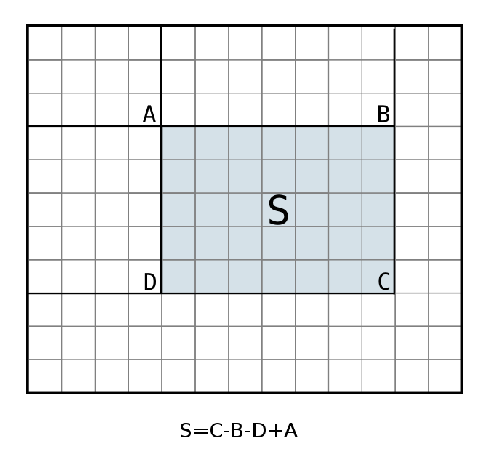
\includegraphics[scale=0.6]{./figs/sumintegralimages2}
	  \caption[Suma de intensidades usando imágenes integrales]{Suma de intensidades en un rectángulo usando imágenes integrales.}
	\label{fig:integral_image_sum}                %% Etiqueta para la figura entera
      \end{figure}

%       La utilización de esta técnica, resulta en un algoritmo invariante a tiempos de cálculo ante cambios del tamaño del filtro, lo cual lo hace particularmente útil cuando se presentan imágenes de grandes dimensiones.   
  En las secciones siguientes, se presenta en detalle los pasos mediante los que se lleva a cabo la detección y descripción de características mediante SURF, introduciendo brevemente el concepto de invarianza a escala.
  \subsection[El problema de cambio de escala]{El problema de cambio de escala en correspondencias de puntos}
    \label{sec:problema_cambio_escala}
    Cuando se trata de hacer coincidir características entre imágenes (por ejemplo para el reconocimiento de las mismas), el problema del cambio de escala se hace presente. Al ser analizadas distintas imágenes, éstas pueden estar tomadas a diferentes distancias respecto del objeto de interés, de forma que los objetos aparecen de diferentes tamaños en la imagen. Luego, si se trata de hacer coincidir las mismas características entre dos imágenes usando un tamaño fijo de píxeles vecinos, la intensidad de los patrones no coincidirá debido al cambio de escala presente en las mismas y por lo tanto, el reconocimiento fallará.

    Para solucionar este problema, el concepto de características invariantes a la escala es introducido en visión computacional, en el que la idea central radica en tener un factor de escala asociada con cada punto clave detectado.
    
    Para comprender mejor esta situación, en la Fig. \ref{fig:church_difference_surf} se presenta un ejemplo de puntos claves detectados con el método SURF. Si se considera la parte inferior de la ventana superior derecha de la fotografía, tanto en la Fig. \ref{fig:church1} como en la Fig. \ref{fig:church2}, la característica SURF ha sido detectada en la misma ubicación y los círculos correspondientes (de diferentes tamaños) contienen los mismos elementos visuales. En la Fig. \ref{fig:church1} la cámara se encuentra más cerca de la escena y el círculo marcado con la flecha roja posee la misma información visual que en la Fig. \ref{fig:church2} donde la escena fue capturada a diferente escala (alejándose la cámara de la escena). % El cambio del tamaño de los círculos correspondientes en ambas imágenes resulta proporcional al cambio de escala. 
    Si bien, en este caso no se da para todas las características, la razón de repetición es lo suficientemente alta para permitir buenas coincidencias entre las dos imágenes. Además, como información adicional, se puede observar una línea radial dentro de cada círculo que indica una orientación asignada a cada punto.% confiriendo invarianza a rotación.
  \subsubsection{Invarianza a escala}%http://fierdetregauche.wordpress.com/2011/03/28/espacio-escala-en-imagenes/
      \label{sec:invarianza_a_escala}
      Es sabido que los filtros gaussianos son comúnmente usados para detección de puntos \cite{Bay:2008:SRF}. Si la escala del filtro es muy pequeña, el resultado incluye muchos puntos redundantes de detalles innecesarios. Contrariamente, si la escala es muy grande, los puntos de regiones con soporte pequeño tienden a desaparecer con el borroneado. Luego, para solucionar los problemas existentes en el filtrado gaussiano con escalas fijas, se han propuesto procedimientos espacio-escala basados en la representación de la curvatura discreta multi escalar. El esquema está basado en el criterio de estabilidad que establece que la presencia de una esquina debe ocurrir como un máximo de curvatura observable en la mayoría de las escalas \cite{springerlink:10.1023/A:1008045108935}.

      La derivada de una imagen puede ser estimada mediante el uso de filtros gaussianos. Los mismos utilizan un parámetro $\sigma$ que representa la varianza de la función gaussiana usada para construir el filtro y que define implícitamente la escala en que la derivada es evaluada.

      Si se calcula el laplaciano de un punto en una imagen usando filtros gaussianos a diferentes escalas, se obtienen diferentes valores en los que se puede observar la evolución de las respuestas para diferentes factores de escala. Así, se  obtiene una curva que alcanza un valor máximo en algún valor de $\sigma$ específico. Si se extrae este valor para dos imágenes del mismo objeto (tomadas a escalas diferentes), la relación que existe entre los $\sigma$ máximos se corresponderán en relación con las escalas en que fueron tomadas cada una de las fotografías. Esta observación es el núcleo del proceso de extracción de características invariantes a la escala que es aplicado tanto en SIFT como en SURF. %Es decir, que las características invariantes a escalas, pueden ser detectadas como máximos locales en ambos espacios. %: espacial (en la imagen) y el espacio escala obtenido de la aplicación de filtros a diferentes escalas.
  \begin{figure}[tbhp]
	\centering
	%%----primera subfigura----
	\subfloat[]{
	      \label{fig:church1}         %% Etiqueta para la primera subfigura
	      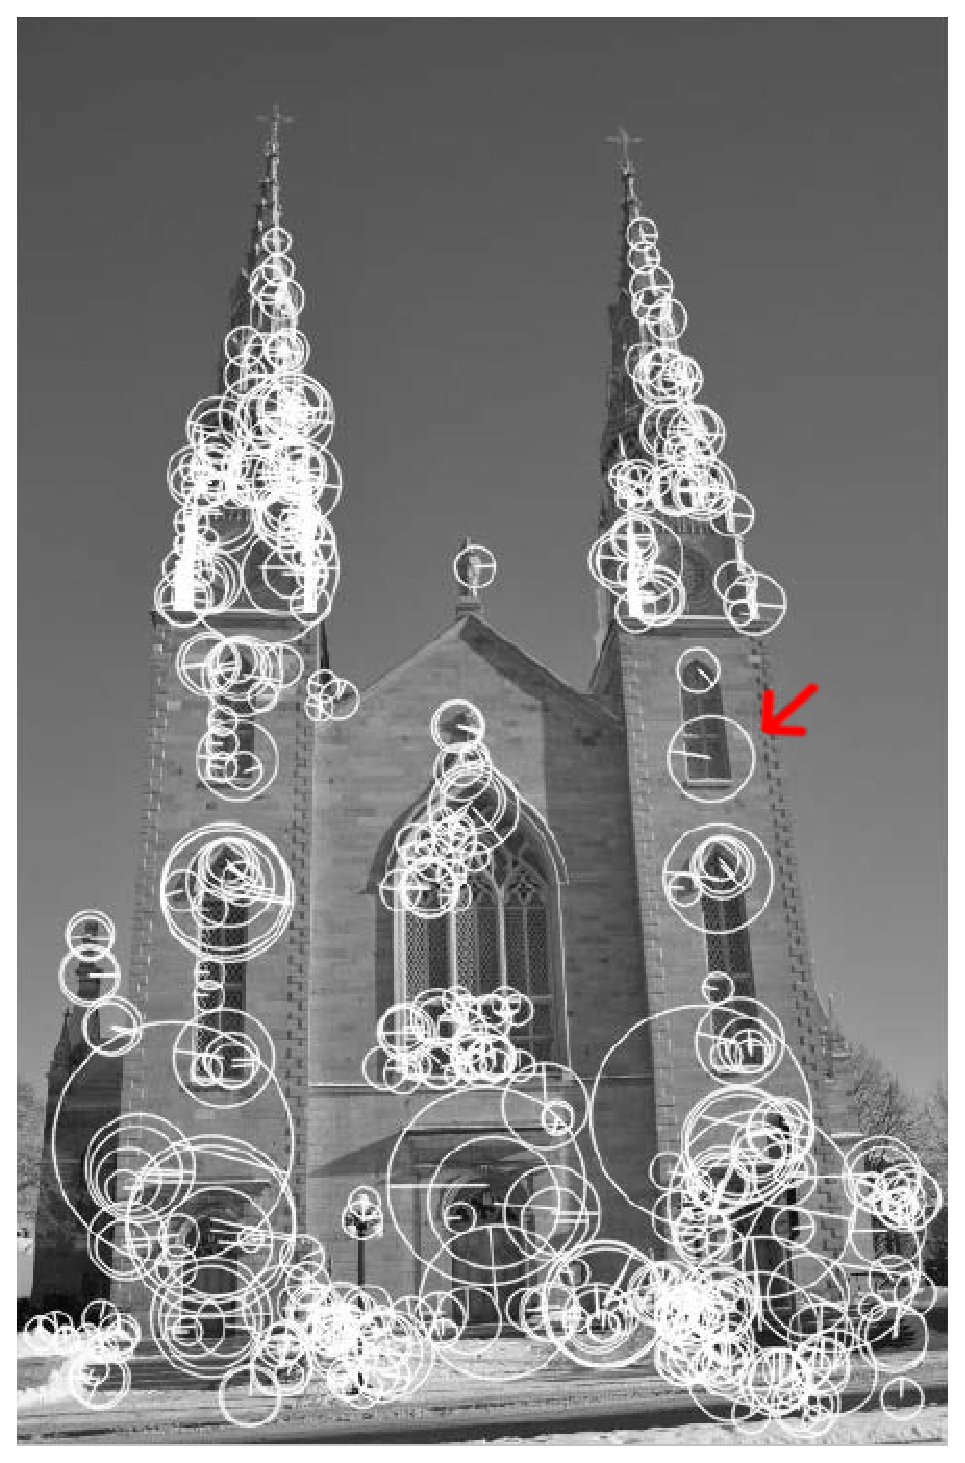
\includegraphics[scale=0.338]{../img_ent2/surfinchurch1}}
	\hspace{0.1\linewidth}
	%%----segunda subfigura----
	\subfloat[]{
	      \label{fig:church2}         %% Etiqueta para la segunda subfigura
	      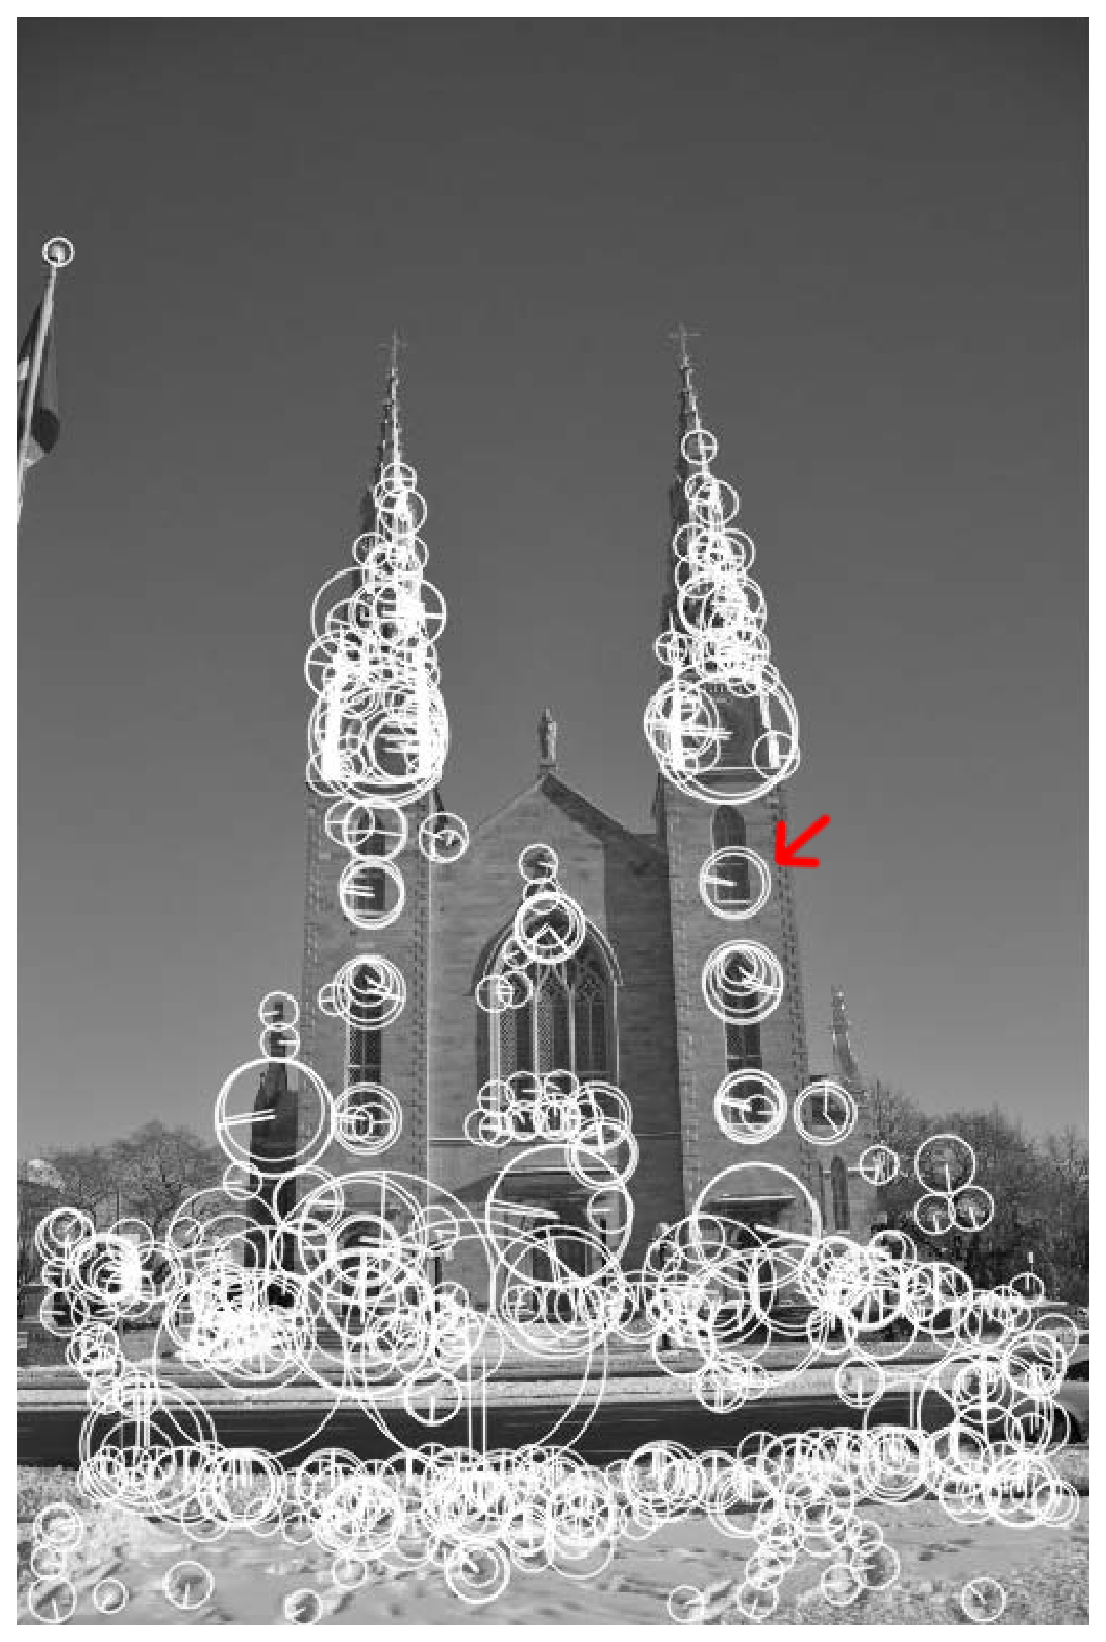
\includegraphics[scale=0.3]{../img_ent2/surfinchurch2}}
	  \caption[Fotografía tomada a diferentes escalas para la misma escena]{Fotografía tomada a diferentes escalas de la misma escena. El tamaño de los círculos de cada punto clave detectado es proporcional a la escala calculada para cada uno de ellos. (Figuras tomadas de \cite{citeulike:9456628}).}
	\label{fig:church_difference_surf}                %% Etiqueta para la figura entera
      \end{figure}
  \subsection{Puntos claves basados en la matriz hessiana}
      \label{sec:matHessiana}
      Con la idea que se introdujo en la sección \ref{sec:problema_cambio_escala}, el descriptor SURF hace uso de la matriz hessiana \eqref{eq:HessianMatrix} y describe cómo las intensidades de los píxeles se distribuyen dentro de una vecindad, que es dependiente de la escala de cada punto de interés detectado por el hessiano. Más específicamente, utiliza el determinante de la matriz para la determinación de la localización y escala de los puntos. Así, cuando el determinante del hessiano es un máximo local (previa eliminación de mínimos mediante un umbral), se determina un punto clave. El uso del hessiano es alentado por su velocidad de cálculo y precisión.%este es el thresholdumbral usado en la funcion %Se puede interpretar que esta matriz mide la curvatura local de una función, mientras que el determinante de la misma da idea de la intensidad que posee la curvatura.
%       La idea es por lo tanto, definir esquinas de imágenes como puntos con con alta curvatura local (esto es, alta variación en más de una dirección)
      \begin{equation}
	H(x,y)=\begin{bmatrix}\frac{\partial^{2}I}{\partial x\text{\texttwosuperior}} & \frac{\partial^{2}I}{\partial x\partial y}\\
	& \\
	\frac{\partial^{2}I}{\partial y\partial x} & \frac{\partial^{2}I}{\partial y\text{\texttwosuperior}}
	\end{bmatrix};\; \textrm{con}\; \frac{\partial^{2}I}{\partial x\partial y}=\frac{\partial^{2}I}{\partial y\partial x}.
	\label{eq:HessianMatrix}
      \end{equation}

      Sea $\mathbf{p}=(x,y)$ un punto en la imagen $\mathit{I}$, la matriz hessiana en $\mathbf{p}$ en la escala $\sigma$ viene definida como:
      \begin{equation}
      \mathcal{H}(\mathbf{p},\sigma)=\left[\begin{array}{cc}
      \mathit{L_{xx}(\mathbf{p},}\sigma)\hphantom{} & \mathit{L_{xy}(\mathbf{p},}\sigma)\\
      \mathit{L_{xy}(\mathbf{p},}\sigma)\hphantom{} & \mathit{L_{yy}(\mathbf{p},}\sigma)
      \end{array}\right],
      \end{equation}
      donde $\mathit{L_{xx}(\mathbf{p},}\sigma)$ es la convolución de la derivada segunda de una gaussiana $\frac{\partial^{2}}{\partial x^{2}}\mathit{g}(\sigma)$ con la imagen $\mathit{I}$ en el punto $\mathbf{p}$; $\mathit{L_{xy}(\mathbf{p},}\sigma)$ es la convolución de la derivada segunda de una gaussiana $\frac{\partial^{2}}{\partial x \partial y}\mathit{g}(\sigma)$ con la imagen $\mathit{I}$ en el punto $\mathbf{p}$ y $\mathit{L_{yy}(\mathbf{p},}\sigma)$ es la convolución de la derivada segunda de una gaussiana $\frac{\partial^{2}}{\partial y^{2}}\mathit{g}(\sigma)$ con la imagen $\mathit{I}$ en el punto $\mathbf{p}$.

      A pesar de que los filtros gaussianos pueden ser utilizados para el análisis del espacio escala como se introdujo en la Sec. \ref{sec:invarianza_a_escala}, SURF hace uso de los filtros tipo caja \cite{conf/nips/SimardBHL98}. Éstos son una aproximación a las derivadas gaussianas segundas y pueden ser aplicados rápidamente cuando se utilizan con las imágenes integrales. Aquí es donde se encuentra presente una de las diferencias que contribuye a una mejora en velocidad del método SURF respecto a SIFT, pues en este último el espacio escala es creado a partir de imágenes suavizadas repetidamente mediante un filtro gaussiano que luego, son submuestreadas (produciéndose un efecto de aliasing indeseado) para alcanzar escalas mayores. En el caso de SURF, el espacio escala es analizado mediante el incremento en el tamaño del filtro. % que independientemente de su tamaño puede ser aplicado a la misma velocidad sobre la imagen original debido al uso de imágenes integrales y filtros tipo caja. 
      Un esquema del espacio escala SIFT puede verse en la Fig. \ref{fig:pyramidfilters} (izquierda) en el que se redimensiona la imagen para obtener las escalas sucesivas; mientras que en el espacio escala SURF en la Fig. \ref{fig:pyramidfilters} (derecha) el redimensionamiento se produce sobre el filtro tipo caja y la imagen es siempre la misma.
      \begin{figure}[tbhp]
	\centering
	      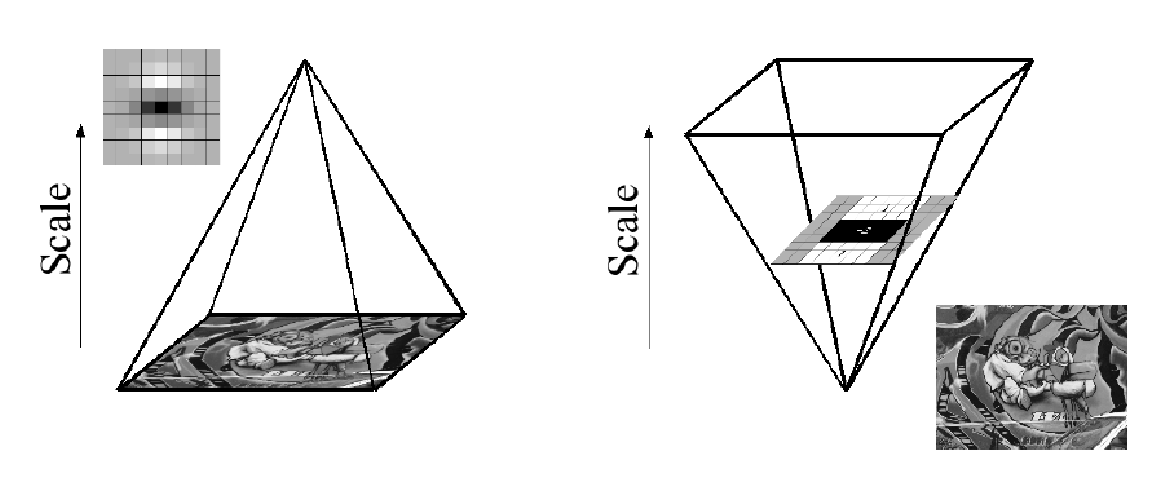
\includegraphics[scale=0.6]{./figs/pyramidfilters}
	  \caption[Pirámide de escala de imágenes para SIFT y SURF]{Pirámide de escala de imágenes para el método SIFT (izquierda) y el método SURF (derecha). (Figura tomada de \cite{Bay:2008:SRF}).}
	\label{fig:pyramidfilters}          %% Etiqueta para la figura entera
      \end{figure}

      Así el determinante de la matriz hessiana (aproximado) usado por SURF queda definido como:
\begin{equation}
      \label{eq:det_happrox}
      \det(\mathcal{H}_{approximado})=D_{xx}D_{yy}-(wD_{xy})^{2} 
      \end{equation}
con $w=0.9$ y donde $\mathit{D}_{xx}$, $\mathit{D}_{yy}$ y $\mathit{D}_{xy}$ son las derivadas parciales gaussianas de segundo orden aproximadas. La ponderación relativa $w$ de la respuesta del filtro es usada para balancear la expresión del determinante hessiano. Si bien el mismo varía para diferentes escalas, en la práctica se puede establecer este factor como constante con $w=0.9$, ya que el mismo no tiene un impacto significante en los resultados \cite{Bay:2008:SRF}.

La derivada parcial de segundo orden gaussiana en la dirección ``y'' $L_{yy}$ puede ser observada en la Fig. \ref{fig:gaussiankernelsdiscreted_y} y su homóloga aproximada $D_{yy}$ en la Fig. \ref{fig:gaussiankernelsaprox_y}; en tanto que en la Fig. \ref{fig:gaussiankernelsdiscreted_xy} se encuentra representada la derivada parcial de segundo orden gaussiana en la dirección ``x-y'' $L_{xy}$ y su homóloga aproximada $D_{xy}$ (Fig. \ref{fig:gaussiankernelsaprox_xy}).
\begin{figure}[tbhp]
	    \centering
	    %%----primera subfigura----
	    \subfloat[]{
		  \label{fig:gaussiankernelsdiscreted_y}         %% Etiqueta para la primera subfigura
		  \includegraphics[scale=0.45]{../img_ent2/gaussiankernelsdiscrete_y}}
		  \hspace{0.1\linewidth}
	    %%----segunda subfigura----
	    \subfloat[]{
		  \label{fig:gaussiankernelsaprox_y}         %% Etiqueta para la segunda subfigura
		  \includegraphics[scale=0.45]{../img_ent2/gaussiankernelsaprox_y}}
		  \hspace{0.1\linewidth}
	    %%----tercera subfigura----
	    \subfloat[]{
		  \label{fig:gaussiankernelsdiscreted_xy}         %% Etiqueta para la segunda subfigura
		  \includegraphics[scale=0.45]{../img_ent2/gaussiankernelsdiscrete_xy}}
		  \hspace{0.1\linewidth}
	    %%----cuarta subfigura----
	    \subfloat[]{
		  \label{fig:gaussiankernelsaprox_xy}         %% Etiqueta para la segunda subfigura
		  \includegraphics[scale=0.45]{../img_ent2/gaussiankernelsaprox_xy}}
		  \hspace{0.1\linewidth}
	  \caption[Derivadas parciales gaussianas discretas y aproximadas]{Derivadas parciales gaussianas de segundo orden discretas y sus homólogas aproximadas (también referenciadas como filtros tipo caja). Las regiones grises de la imagen son iguales a cero (Figuras tomadas de \cite{Bay:2008:SRF}).}%% Etiqueta para la figura entera
	    \label{fig:gaussiankernels}
      \end{figure}
      %
      Como se ha mencionado, en el método SURF se aplican sucesivamente filtros de tamaño creciente sobre la imagen original. El filtro más pequeño utilizado tiene un tamaño de $9 \times 9$ y corresponde a la derivada parcial de segundo orden de una gaussiana con $\sigma=1.2$ siendo este el nivel de escala inicial que da la máxima resolución espacial ($s=1.2$). De la misma forma, convolucionando la imagen original con filtros de mayores dimensiones se van obteniendo los niveles siguientes.

      El espacio escala para el descriptor SURF está dividido en octavas. Una octava representa una serie de respuestas obtenidas mediante la convolución de la imagen original con filtros de tamaños cada vez mayores. En total, una octava comprende un factor de escalado de 2 y cada una de ellas es subdividida en un número constante de niveles de escala (véase la Fig. \ref{fig:maximum_supression3by3by3}).
 En la Fig. \ref{fig:tamfilters1} se puede observar un esquema gráfico del análisis de 3 octavas en donde el eje horizontal, expresado logarítmicamente, representa las escalas. Notar que para cada nueva octava, el tamaño del filtro es incrementado al doble (en la primer octava el paso es 6, en la segunda de 12, en la tercera 24, etc.) y cada una de ellas empieza con un tamaño de filtro igual al segundo de la octava anterior. También, se puede observar que las octavas están solapadas, esto, con el objetivo de cubrir todas las posibles escalas. %Se hace notar para el método que cuanto más octavas son procesadas el número de puntos detectado por octavas decae rápidamente. 
 Por ejemplo, para la primer octava el espacio escala comienza con filtros de $9 \times 9$ continuando con los de $15 \times 15$, $21 \times 21$, y $27 \times 27$. Debido a que se realiza una supresión de no-máximos\footnote{La supresión de no-máximos fija en cero a todos los píxeles de una vecindad que son menores al máximo valor presente en la misma. También se utiliza el término filtro de máxima para referirse a este concepto.} tanto espacialmente como con las escalas vecinas, las respuestas del hessiano en el primer y último nivel son usadas solo para comparación. Por ello, luego de realizar una interpolación, la escala posible más pequeña es $\sigma = 1.6$ correspondiente a un filtro de $12 \times 12$, y la más grande a $\sigma = 3.2$ correspondiente a un filtro de $24 \times 24$. Consideraciones similares se aplican para las demás octavas. Para más detalles se puede consultar \cite{DBLP:phd/ch/Bay2009}.
      \begin{figure}[tbhp]
	\centering
	      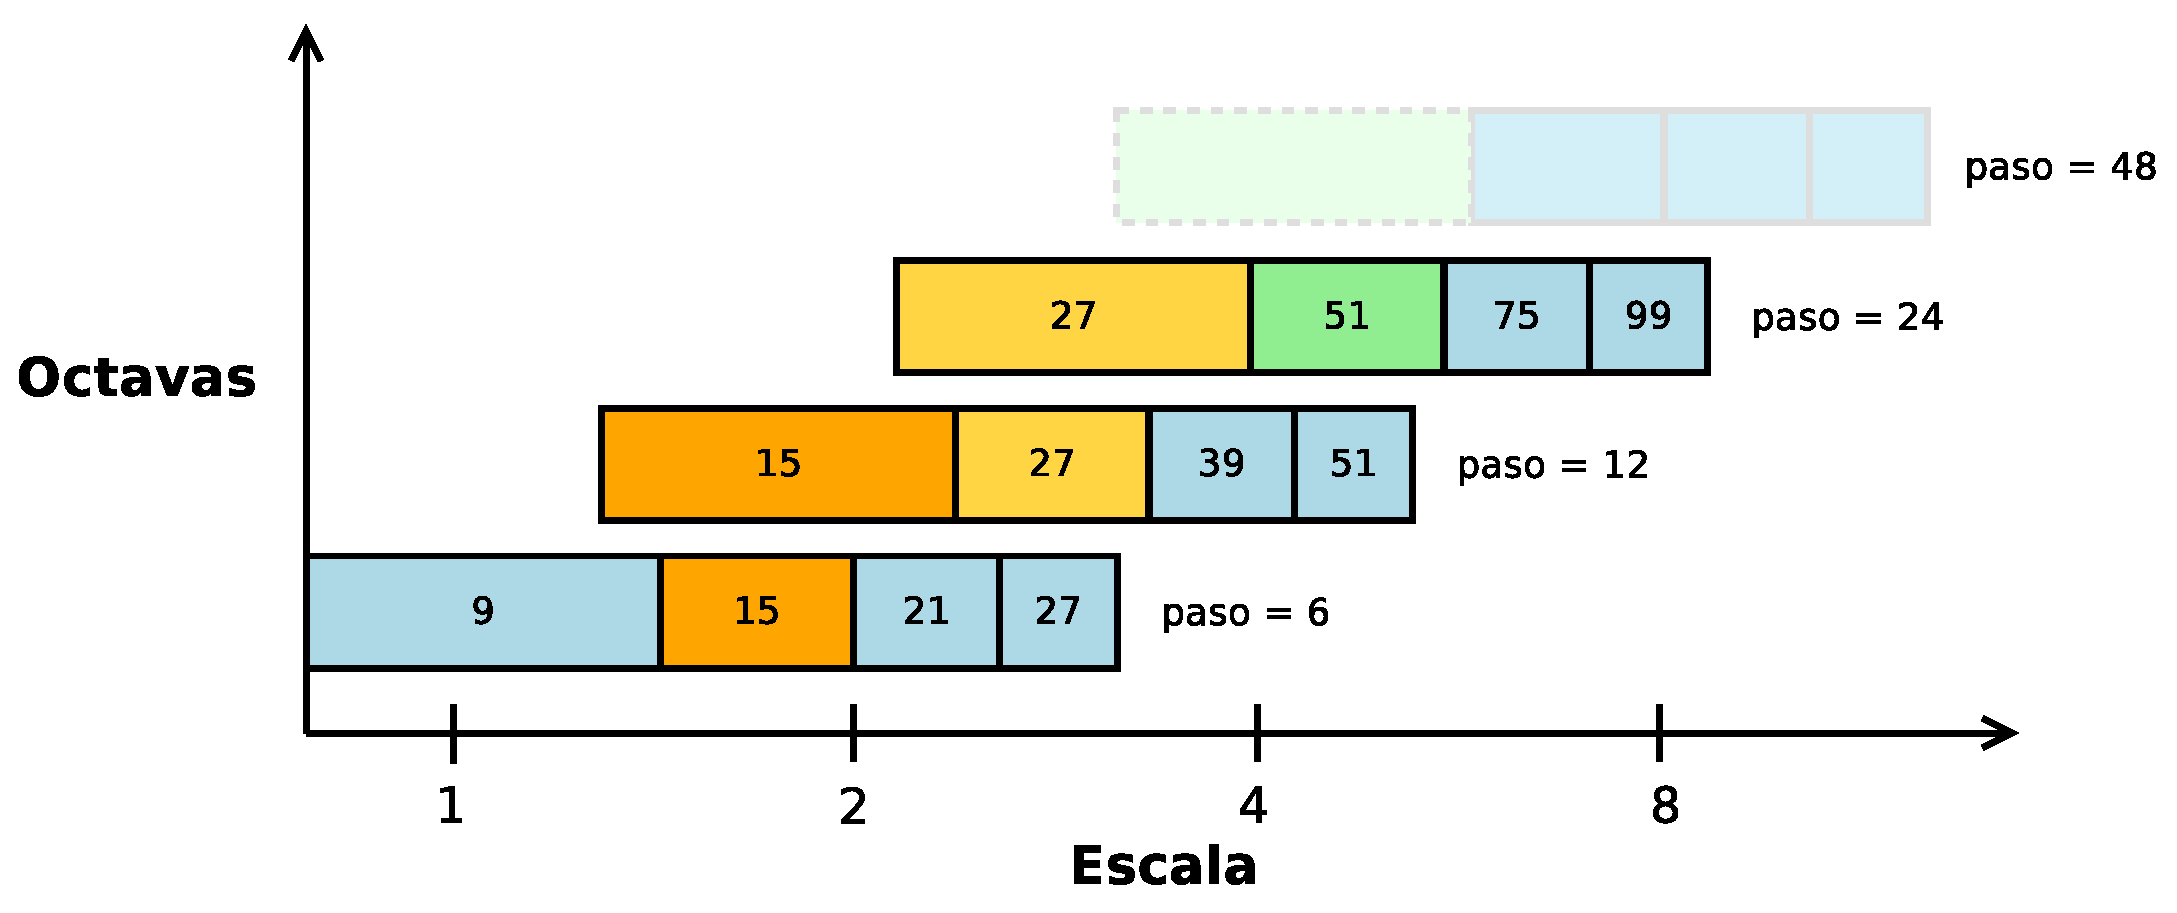
\includegraphics[scale=0.32]{./figs/tamfilters1}
	  \caption[Longitudes de los filtros para 3 diferentes octavas]{Representación gráfica de las longitudes de los filtros para 3 diferentes octavas (Figura adaptada de \cite{Bay:2008:SRF}).}
	\label{fig:tamfilters1}               %% Etiqueta para la figura entera
      \end{figure}
      \subsection{Determinación de la localización de puntos claves} %http://es.wikipedia.org/wiki/Reconocimiento_de_regiones
    Como se ha visto en la sección anterior, se construye una ``pirámide de respuestas'' con diferentes niveles de escalas dentro de las octavas. La localización de los puntos claves como su escala, se determinan hallando los extremos entre los 8 vecinos en el nivel evaluado y los $2 \times 9$ vecinos en el nivel inmediatamente superior e inferior mediante la supresión de no-máximos en la vecindad de $3 \times 3 \times 3$. Un esquema puede ser observado en la Fig. \ref{fig:maximum_supression3by3by3} donde se demarca dicha vecindad.
      \begin{figure}[tbhp]
	\centering
	      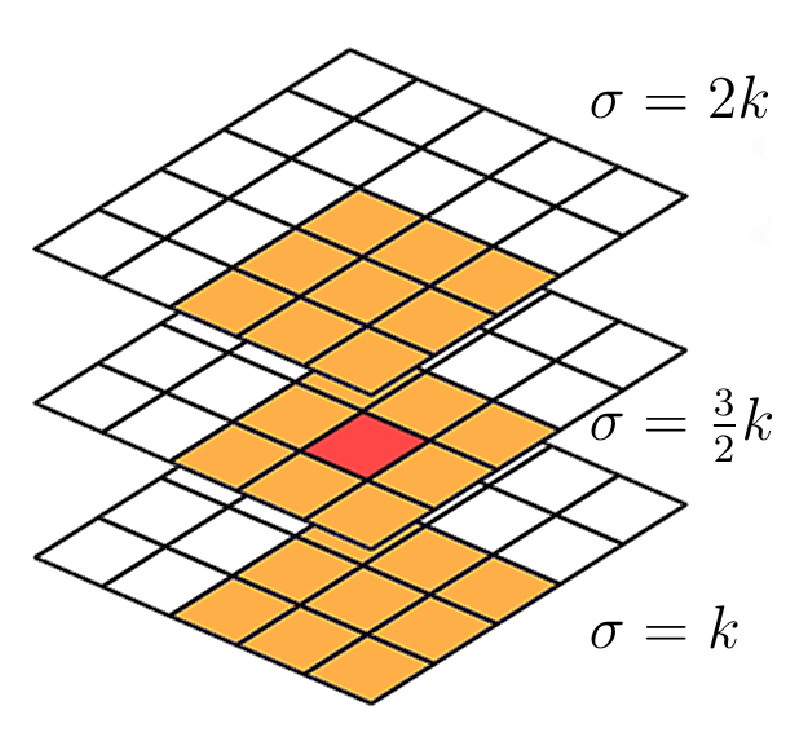
\includegraphics[scale=0.35]{./figs/333nonmaximum}
	  \caption[Representación de una octava compuesta por tres niveles de escala]{Representación de una octava compuesta por tres niveles de escala $\sigma=k$, $\sigma=\frac{3}{2}k$, $\sigma=2k$.}
	\label{fig:maximum_supression3by3by3}               %% Etiqueta para la figura entera
      \end{figure}

      	Una vez que el máximo local es identificado, la posición precisa de cada punto clave es obtenida a través de interpolación y el resultado es un conjunto de puntos claves localizados con precisión sub-píxel, los cuales están asociados a un valor de escala \cite{DBLP:phd/ch/Bay2009}.
      	
%       	Para encontrar la ubicación interpolada del punto de interés, se tienen en cuenta los máximos en la vecindad de $3 \times 3 \times 3$ en cada dimensión alrededor del máximo detectado como se ha descripto arriba. Luego se localiza el máximo mediante el ajuste de una función cuadrática 3D en el espacio escala sobre el las respuestas.
	 %De esta manera, el máximo determinante de la matriz Hessiana es interpolado en la escala y posición de la imagen. %usando 4 octavas, 8 escalas son analizadas	
% 	Cuando la búsqueda de extremos se produce en las octavas más altas, el área cubierta por los filtros resulta de un tamaño considerable y esto introduce un error significativo al momento de determinar la posición de los puntos de interés. Para solucionar este inconveniente, la determinación de la posición del punto de interés es interpolada mediante el ajuste a una función cuadrática 3D en el espacio escala mediante expansión en series de Taylor \cite{Brown02invariantfeatures}. 
% 	
% 	Así, se expresa el Hessiano como una función $H(x,y,\sigma)$ mediante la descomposición en series de Taylor \eqref{eq:expansionTaylorSeries}
% 	 para buscar los extremos estableciendo la derivada a cero y resolviendo la ecuación \eqref{eq:equationinterpolation} para encontrar $\mathbf{\hat{p}}=(x,y,s)$
% 	\begin{equation}
% 	 \label{eq:expansionTaylorSeries}
% 	 H(\mathbf{p})=H+\frac{\partial H^{\mathtt{T}}}{\partial\mathbf{p}}\mathbf{p}+\frac{1}{2}\mathbf{p}^{\mathtt{T}}\frac{\partial^{2}H^{\mathtt{T}}}{\partial\mathbf{p}^{2}}\mathbf{p}
% 	\end{equation}
% 	\begin{equation}
% 	 \label{eq:equationinterpolation}
% 	 \mathbf{\hat{p}}=\frac{\partial^{2}H^{-1}}{\partial\mathbf{p}^{2}}\,\frac{\partial H}{\partial\mathbf{p}}
% 	\end{equation}
% 	
% 	De esta forma se obtiene la ubicación de un punto de interés asociados a un valor de escala.%\cite{DBLP:phd/ch/Bay2009}
%       Una característica invariante a la escala es identificada cuando el determinante del Hessiano alcanza un máximo local en ambos espacios imagen y escala (esto es, 3x3x3 supresión de no-maximos es necesario llevar a cabo). Debemos aclarar que previamente se define un umbral mínimo para determinar cuales son los máximos que participan en la selección final.

\section{Descripción de puntos claves}
    \label{sec:descripcion_ptos_claves}
    Tras la localización y la asociación de escala a los puntos claves, la siguiente etapa consiste en asignar una orientación a cada uno de ellos para otorgarles invarianza ante la rotación mediante la orientación del mismo.
%   El descriptor SURF describe la distribución de las intensidades en una vecindad del punto clave construyendose sobre la distribución de las respuestas de las wavelets Haar de primer orden y utilizando imágenes integrales para aumentar la velocidad.
%   
%   El primer paso consiste en fijar una orientación basada en la información de una región circular alrededor del punto de interés detectado. Luego se construye una región cuadrada alineada con la orientación seleccionada y se extrae el descriptor SURF de la misma.
  \subsection{Asignación de la orientación}
    \label{sec:orientacion_del_punto}
     Para definir la orientación, primeramente se calculan las respuestas con los filtros presentados en la Fig. \ref{fig:simplekernels} sobre un área circular de radio $6s$ alrededor del punto clave, siendo $s$ la escala en que se detectó el punto. Tanto el muestreo como el tamaño de los filtros son dependientes de la escala y se establecen a $s$ y $4s$ respectivamente (a mayor escala, mayor es la dimensión de las wavelets). %(longitud del lado)
    La evaluación de los filtros realizada aquí, se vale nuevamente de las imágenes integrales para realizar los cálculos más rápidamente. Tras el cálculo de las respuestas, las mismas son ponderadas con una gaussiana de valor $\sigma=2s$ centrada en el punto clave.  
    \begin{figure}[tbhp]
       \centering
       %%----primera subfigura----
       \subfloat[]{
            \label{fig:simplekernels1}         %% Etiqueta para la primera subfigura
            \includegraphics[scale=0.4]{../img_ent2/simplekernels1harn}}
       \hspace{0.1\linewidth}
       %%----segunda subfigura----
       \subfloat[]{
            \label{fig:simplekernels2}         %% Etiqueta para la segunda subfigura
            \includegraphics[scale=0.4]{../img_ent2/simplekernels2harn}}
        \caption[Filtros Wavelets Haar]{Filtros Wavelets Haar para calcular las respuestas en la dirección $x$ \subref{fig:simplekernels1} e $y$ \subref{fig:simplekernels2}.}
       \label{fig:simplekernels}                %% Etiqueta para la figura entera
    \end{figure}
    
    Luego, las respuestas son representadas como puntos en el espacio (respuestas horizontales a lo largo del eje de abscisas $dx$ y verticales $dy$ en el de ordenadas) y la orientación dominante se determina mediante la suma de todas las respuestas en una ventana deslizante orientada de tamaño $\pi/3$, como puede observarse en la Fig. \ref{fig:responsecalculate}. Así, las respuestas horizontales y verticales dentro de la ventana son sumadas constituyendo un vector de orientación local. La orientación final para el punto clave, es aquella en la que el vector resulta ser el más largo entre todas las ventanas.
% 
%  una ventada deslizante orientada de tamaño $\frac{\pi}{3}$ detecta la orientación dominante de la respuesta de las wavelets haar ponderadas con un gaussiano en una vecindad circular alrededor del punto clave. Las dirección de respuesta horizontal y vertical están representadas por los puntos en los ejes $dx$ y $dy$ respectivamente. 
    \begin{figure}[tbhp]
      \centering
	    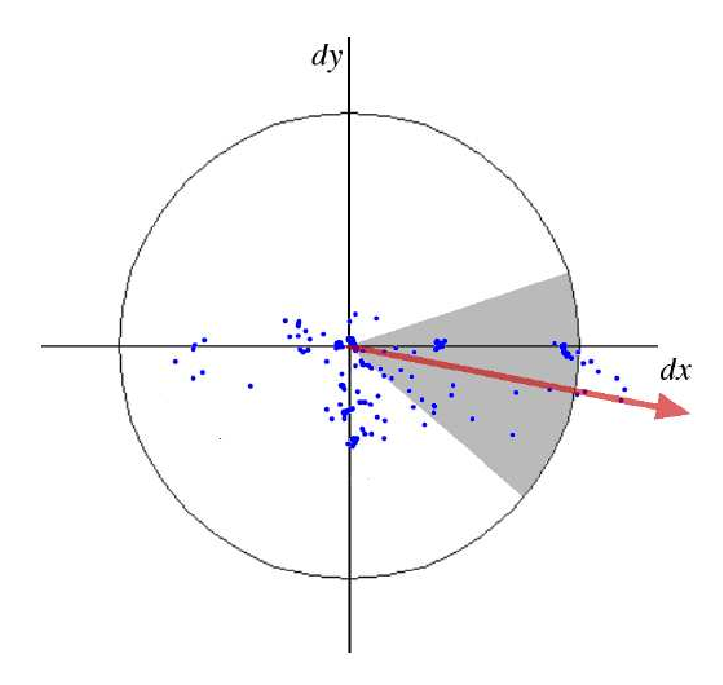
\includegraphics[scale=0.45]{./figs/responsecalculate}
	\caption[Asignación de la orientación para un punto clave]{Asignación de la orientación para un punto clave con una ventana deslizante orientada de tamaño $\frac{\pi}{3}$. (Figura tomada de \cite{Bay:2008:SRF}).}
      \label{fig:responsecalculate}                %% Etiqueta para la figura entera
    \end{figure}
   \subsection{Creación del descriptor}
      En esta última parte, se termina la creación del descriptor SURF.
      El primer paso consiste en construir una región cuadrada de tamaño $20s$ centrada en el punto de interés y orientada de acuerdo al resultado que se obtuvo en la sección \ref{sec:orientacion_del_punto}. Ejemplos de esas regiones cuadradas son ilustradas en la Fig. \ref{fig:squareregionsexample}.
      \begin{figure}[tbhp]
	\centering
	      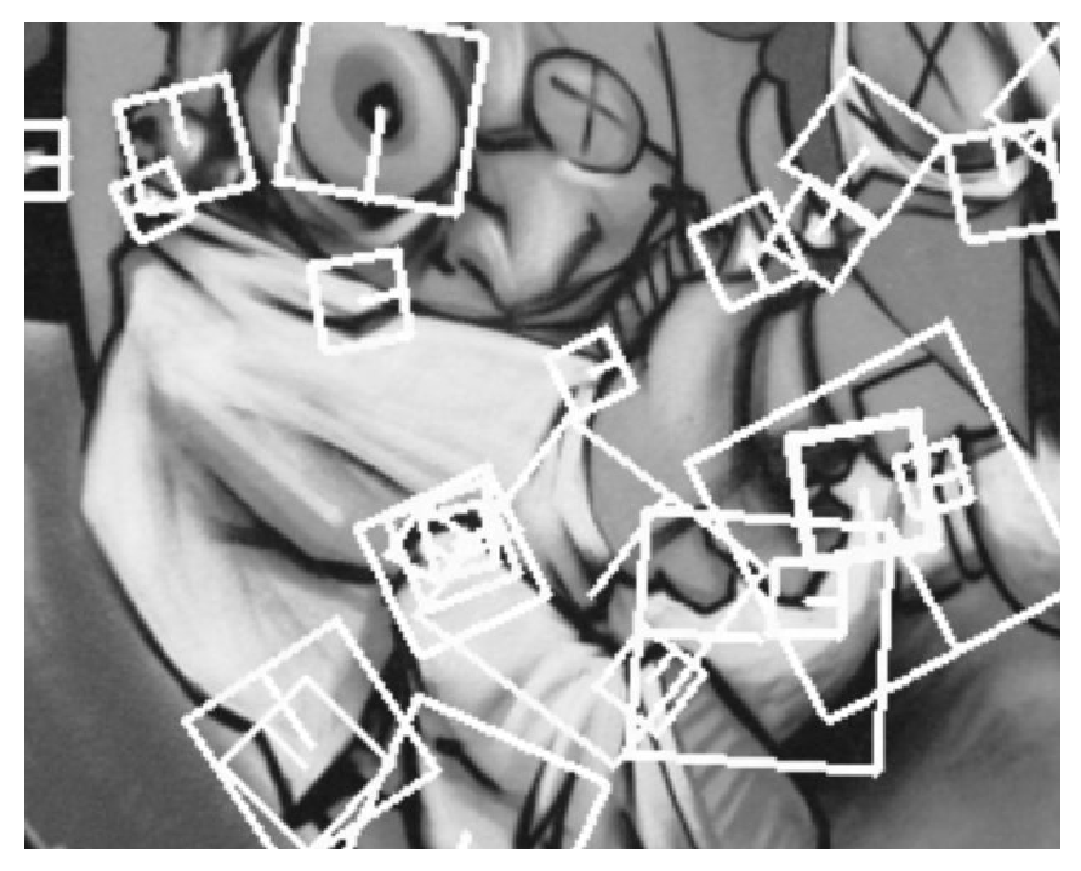
\includegraphics[scale=0.4]{./figs/squareregionsexample}
	  \caption[Ejemplo de ventanas del descriptor a diferentes escalas sobre una imagen]{Detalle de una escena mostrando el tamaño de las ventanas orientadas del descriptor a diferentes escalas. (Figura tomada de \cite{Bay:2008:SRF}).}
	\label{fig:squareregionsexample}                %% Etiqueta para la figura entera
      \end{figure}
      \begin{figure}[tbhp]
	\centering
	%%----primera subfigura----
	\subfloat[]{
	      \label{fig:subdivideregions}         %% Etiqueta para la primera subfigura
	      \includegraphics[scale=0.30]{./figs/subdivideregions}}
	\hspace{0.1\linewidth}
	%%----segunda subfigura----
	\subfloat[]{
	      \label{fig:left_boxfilters}         %% Etiqueta para la segunda subfigura
	      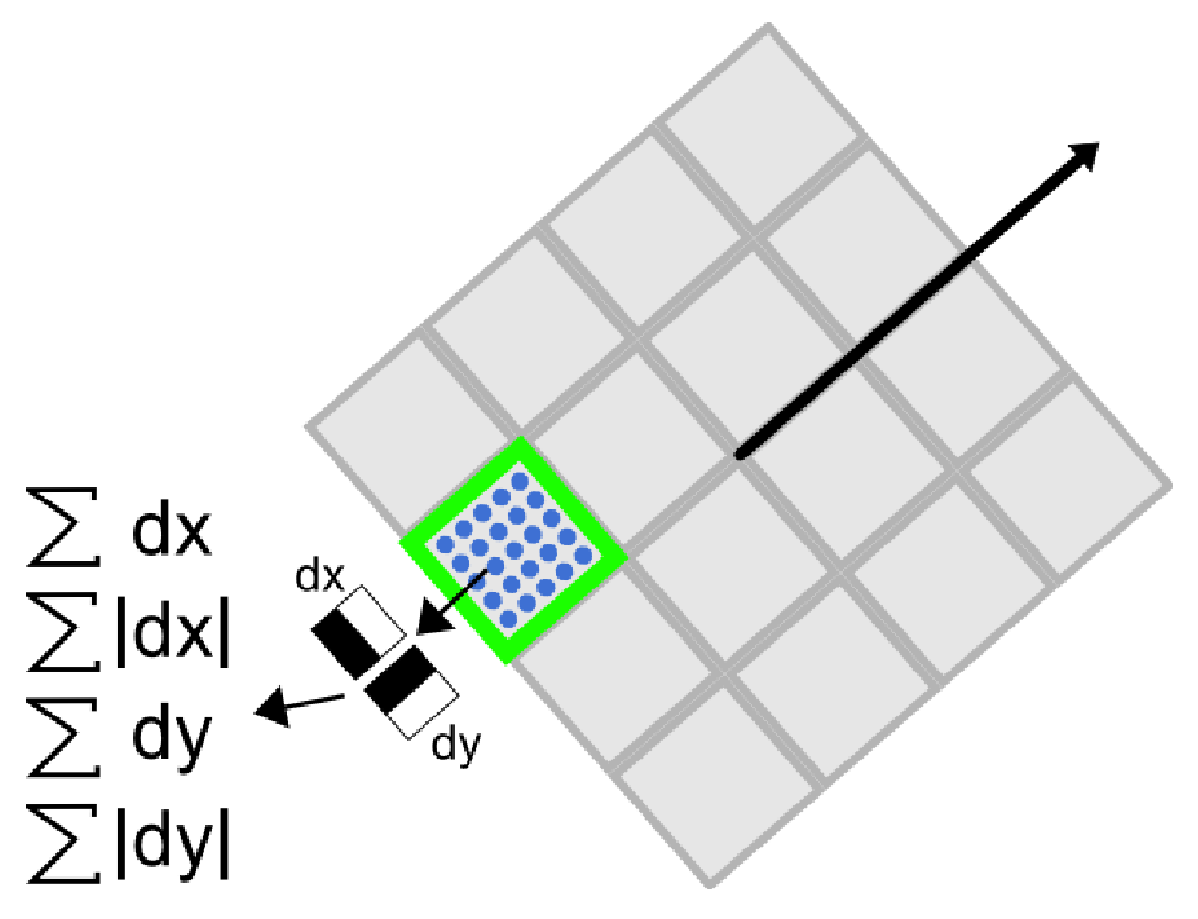
\includegraphics[scale=0.30]{./figs/respuestaswavelethaar}
	  }
	\label{fig:regioneshaarandresponses}                %% Etiqueta para la figura entera
	\caption[Interpretación gráfica del descriptor SURF]{Interpretación gráfica del descriptor SURF. (Figuras tomadas de \cite{Bay:2008:SRF}).}
      \end{figure}
      \begin{figure}[tbhp]
	\centering
	      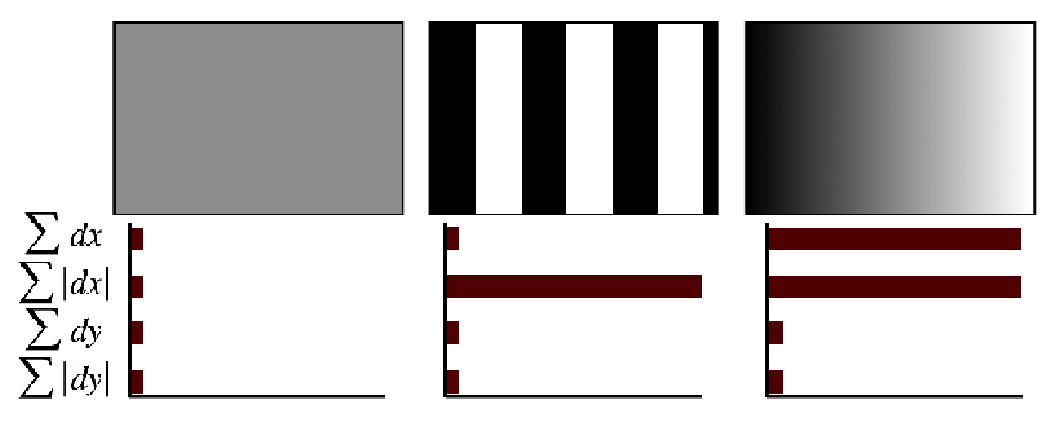
\includegraphics[scale=0.60]{./figs/descriptorresponses}
	  \caption[Descriptores resultantes para tres subregiones con patrones diferentes]{Descriptores resultantes para tres subregiones con patrones diferentes (Figura tomada de \cite{Bay:2008:SRF}).}
	\label{fig:descriptorresponses}                %% Etiqueta para la figura entera
      \end{figure}
      Seguidamente, cada región es dividida en subregiones de $4 \times 4$ como se puede observar en la grilla cuadrada orientada sobre el punto de interés en la Fig. \ref{fig:subdivideregions}. Luego para cada subregión se calculan las respuestas de las waveletes Haar con una separación de muestreo de $5 \times 5$. Las subdivisiones de $2 \times 2$ de cada cuadrado corresponden a los campos reales del descriptor que son las sumas $dx$, $|dx|$, $dy$ y $|dy|$ calculadas relativas a la orientación de la grilla como se observa en la Fig. \ref{fig:left_boxfilters} donde se denota con $d_x$ y $d_y$ a la respuesta de la wavelet Haar en la dirección horizontal y vertical respectivamente (relativas a la orientación del punto clave, con tamaño del filtro igual a $2s$). Se debe tener en cuenta que para incrementar la robustez ante deformaciones geométricas y errores de localización, las respuestas $d_x$ y $d_y$ son primero ponderadas con un gaussiano con $\sigma=3.3s$ centrado en el punto de interés. % Un ejemplo de la subdivisión y el resultado de las respuestas, puede ser observado en la Fig. \ref{fig:subdivideregions}. 
%Finalmente, el descriptor SURF consiste en las respuestas de la wavelet Haar en una región de 4x4 alrededor del punto clave \cite{Evans09noteson}.
      Luego, las respuestas $d_x$ y $d_y$ se suman en cada subregión, como así también los valores absolutos de las mismas $|dx|$ y $|dy|$ con el objetivo de brindar información de la polaridad sobre los cambios de intensidad. De esta forma, cada subregión queda representada por un vector de 4 dimensiones $\mathbf{v}$, que caracteriza su intensidad localmente $\mathbf{v}=(\sum{d_x},\sum{d_y},\sum{|d_x|},\sum{|d_y|})$. Debido a que se tienen $16$ subregiones ($4 \times 4$) con vectores de 4 dimensiones por subregión, se obtiene un vector descriptor de 64 dimensiones ($16 \times 4$) por cada punto clave detectado, por lo que se puede decir que el descriptor SURF consiste en las respuestas de la wavelet Haar en una región de 4x4 alrededor del punto clave \cite{Evans09noteson}. Las repuestas wavelet son invariantes a un sesgo en la iluminación, mientras que la invarianza al contraste es alcanzado mediante la normalización del descriptor.
 %conversión del descriptor a uno unitario.
      
      En la Fig. \ref{fig:descriptorresponses} se pueden observar los descriptores para tres subregiones con patrones de imágenes diferentes. En el caso de una región homogénea se puede observar que todos los valores son relativamente bajos; en presencia de frecuencias en la dirección de $x$, los valores de $\sum{|d_x|}$ son altos, mientras los otros son bajos y si la intensidad se incrementa gradualmente en la dirección $x$, ambos valores $\sum{d_x}$ y $\sum{|d_x|}$ son altos.
%       SURF es, hasta un cierto punto, conceptualmente similar a SIFT, en el sentido de que ambos se enfocan en la información de la distribución espacial del gradiente. Sin embargo, SURF supera a en la práctica a SIFT en todos los casos como se mostrará en la sección \ref{sec:seccion5}. Se cree que esto es debido al hecho de que SURF integra la información del gradiente en un sub parche, mientras que SIFT depende de las orientaciones de los gradientes individuales. Esto hace a SURF menos sensitivo al ruido, como se muestra en la figura \ref{fig:surflesssensitivetonoise}
      
      Si bien existen muchos parámetros del método que pueden variarse, en este capítulo se han expuestos aquellos que el autor \cite{Bay:2008:SRF} recomienda según sus resultados en la publicación original.
%%%%%%%%%%%%%%%
\section{Correspondencia entre puntos claves}
\label{sec:correspop_ptos_claves}
El término correspondencia entre puntos o entre imágenes se puede interpretar como el cálculo de un valor que represente el grado de similitud entre dos imágenes. Para ello, la correspondencia entre los puntos claves de dos imágenes es buscada mediante el cálculo de la distancia euclídea entre los vectores característicos asociados a los puntos claves detectados en cada una de las imágenes. %Este cálculo, genera un valor que es utilizado para determinar la correspondencia entre los puntos de las imágenes que se están comparando.
%Poseer un descriptor de 64 dimensiones para cada punto clave detectado, resulta útil en la medida que se tenga un método para decidir cuando un descriptor de consulta coincide con un descriptor de la imagen patrón. 
Es decir que el problema que se plantea aquí, es el de comparar los descriptores de los puntos claves de las imágenes para determinar coincidencias de puntos y así afirmar o no la presencia del objeto buscado.

El m\'etodo de búsqueda del vecino más cercano (NNS: del inglés, Nearest Neighbor Search) \cite{AryaEtAl98} es un método de gran utilidad. Se ha aplicado a gran variedad de aplicaciones como el reconocimiento de imágenes, la compresión de datos, los sistemas de recuperación de documentos, estadísticas y análisis de datos, entre otros. %Debido a que los puntos se encuentran en un espacio, estos tienen una noción de distancia (eg. la distancia euclidea).
NNS es un problema de optimización que intenta buscar los puntos más cercanos en un espacio métrico: dado un conjunto de puntos $P=\left\{ p_{1,...,}p_{n}\right\}$ en un espacio métrico $M$ y un punto de consulta $q \in M$, encontrar el punto más cercano a $q$ en $P$ de forma eficiente, donde $M$ es un espacio euclídeo d-dimensional y las distancia es medida por ejemplo mediante la distancia euclídea.

Existe una variante al algoritmo NNS denominada k-NN (k-Nearest Neighbor) que a diferencia del anterior, evalúa a qué clase pertenecen los $K$ vecinos más cercanos para decidir la clase. Así, en el caso $K=1$ se está en presencia del algoritmo NNS que se describió anteriormente

% Cada uno de los datos de entrenamiento consiste en un conjunto de vectores con sus clases asociadas con cada vector(Que rempresentaría en mi las clases)
Resolver problemas de búsqueda de vecinos más cercanos, no resulta trivial en espacios de grandes dimensiones \cite{muja_flann_2009}. No es usual encontrar algoritmos que posean un rendimiento mayor al de la búsqueda lineal (también conocida como ``búsqueda por fuerza bruta''), la cual resulta costosa computacionalmente y hasta a veces, imposible de usar en muchas aplicaciones. Es por esto, que se ha generado un gran interés en algoritmos que puedan realizar la búsqueda del vecino más cercano de forma aproximada, con lo cual es posible lograr mejoras significativas en tiempo de ejecución con errores de precisión relativamente pequeños y aceptables \cite{muja_flann_2009, Beis:1997:SIU:794189.794431}. %Para ello, se preprocesan los datos de alguna manera, de tal forma de obtener las coincidencias más rápidamente tratando de perder la menor precisión posible.

En el trabajo de Slipa-Anan y Hartley \cite{Silpa_KDTree, bb77826}, se propuso la creación de una estructura de múltiples árboles KD o K-dimensionales aleatorios conocidos por su término en inglés como \textbf{Randomized KD-Tree}, que brinda la posibilidad de obtener resultados satisfactorios en un amplio rango de problemas \cite{muja_flann_2009}. Más específicamente, para casos en los que se trata con vectores similares a los presentados en la Sec. \ref{sec:descripcion_ptos_claves} resulta una alternativa aceptable. Por ello, se utilizará el método descripto en \cite{Silpa_KDTree, bb77826} con los parámetros estudiados que se describen en \cite{muja_flann_2009}.
\subsection{El algoritmo de árboles KD aleatorio}
El algoritmo KD-tree clásico resulta eficiente con datos de bajas dimensiones \cite{Friedman:1977:AFB:355744.355745}, pero su rendimiento se ve afectado rápidamente al aumentar la dimensionalidad de los datos. 
Para obtener una velocidad mayor a la de la búsqueda lineal, se hace necesario establecer una búsqueda aproximada del vecino más cercano. Esto mejora el tiempo de búsqueda pero, como contrapartida, el algoritmo no siempre da como resultado el vecino más cercano. Para realizar esta búsqueda aproximada de forma rápida, se crea una estructura de árbol que contribuye a la reducción en los tiempos de procesamiento.% Un árbol KD es una estructura de datos jerárquica construida mediante el particionamiento recursivo de los datos a lo largo de la dimensión de mayor varianza usada para resolver rápidamente problemas del vecino más cercano.

Los elementos guardados en el árbol KD-tree, son vectores de altas dimensiones. En la raíz del árbol (primer nivel), los datos son divididos en dos mitades por un hiper plano ortogonal para una dimensión elegida y con un valor de umbral. Generalmente, esta división se realiza con la media, en la dimensión con la mayor varianza del conjunto de datos. En características visuales provistas por SIFT o SURF, utilizar la media en la dimensión con mayor varianza es la que presenta el mejor rendimiento \cite{muja_flann_2009}. Para construir el árbol, se compara el vector de entrada con el ``valor de partición'' para determinar a qué mitad del árbol pertenece dicho vector.
Cada una de las dos mitades de los datos es dividida de igual manera y en forma recursiva, para lograr crear un árbol binario completamente balanceado.
% Cada nodo de la parte inferior del \'arbol corresponde a un punto simple del conjunto de datos. 
% Sin embargo, en algunas aplicaciones los nodos hojas pueden tener más de un punto.
%Slipa-Anan y Hartley \cite{Silpa_KDTree}, han propuesto una versión del algoritmo de árbol KD en el que múltiples árboles KD aleatorios son creados \cite{Silpa_KDTree, bb77826}. 
% Como se ha mencionado, el algoritmo de árboles KD original, divide los datos en mitades %por la mitad 
% en cada nivel del árbol, en la dimensión para la cual los datos exhiben la mayor varianza.

A diferencia del algoritmo KD-tree clásico, los árboles aleatorios son construidos seleccionando la dimensión de división de forma aleatoria sobre las primeras $D$ dimensiones en las que los datos poseen mayor varianza. 
Se usa el valor fijo $D=5$ que resulta el más adecuado para diferentes datos \cite{muja_flann_2009}. %Un ajuste adicional sobre dicho valor, no otorga beneficios importantes.
%en vez de usar x, y, x y para decidir para que lado tira el nodo, saca la varianza en el nivel, selecciona las 5 más variantes y sobre esas aleatoriamente toma una.

Cuando se realiza la b\'usqueda en el árbol, una cola con prioridad es mantenida a través de todos los árboles aleatorios, por lo que la búsqueda queda ordenada mediante el incremento de la distancia a cada nodo del borde. 
El grado de aproximación, se determina mediante el examen de un número fijo de nodos hoja. Cuando es alcanzado este número, se termina la búsqueda y se obtienen los candidatos. 
Se debe tener en cuenta que la cantidad de memoria utilizada aumenta linealmente con el número de árboles aleatorios, una característica negativa cuya importancia no resulta menor en la sobrecarga del sistema.

\subsection{Remoción de correspondencias no válidas}
\label{sec:remocion_corresp_invalidas}
La utilización de la forma de búsqueda de coincidencias descripta en la sección anterior no resulta del todo adecuada, ya que para un punto clave de consulta siempre se encontrarán valores de correspondencias que no necesariamente son válidos. Por ello, se hace necesario la aplicación de un umbral para determinar las potenciales correspondencias válidas. Usar un valor de umbral global que se compare con la distancia a la característica más cercana no funciona correctamente
%, ya que algunos descriptores son más discriminativos que otros 
según lo afirma Lowe \cite{Lowe:2004:DIF:993451.996342}. Por ello, se propone considerar una medida más efectiva obtenida mediante la comparación de la distancia del vecino más cercano respecto del segundo vecino más cercano. Así la estrategia que se propone en \cite{Lowe:2004:DIF:993451.996342} es la utilizada en este trabajo y es la que se describe a continuación.

Sean $A$ y $B$ dos imágenes sobre las cuales se quieren buscar correspondencias. Consideremos $a_i$ con $i=0\ldots n$ un punto del conjunto de puntos claves detectados en $A$, $n$ el total de puntos claves detectados en $A$, $av_i$ el vector característico asociado al punto $a_i$ y de forma similar para la imagen $B$. Para cada $a_i$, se seleccionan los dos mejores puntos claves candidatos $p_1 \in b_i$ y $p_2 \in b_i$ cuyos vectores de características asociados a cada uno representan las distancias euclídeas mínimas $d_1$ y $d_2$ respectivamente respecto a $av_i$. Luego, si se cumple la proporción $\frac{d_{1}}{d_{2}}>\varepsilon\qquad(\varepsilon=0.8\:\cite{Lowe:2004:DIF:993451.996342})$ la coincidencia es rechazada.
El valor de $\varepsilon=0.8$ fue seleccionado de acuerdo al estudio llevado a cabo por Lowe \cite{Lowe:2004:DIF:993451.996342} que afirma que se alcanzan a eliminar un 90\% de falsas coincidencias mientras se descartan sólo un 5\% de buenas coincidencias, resultando en el valor más apropiado. %Valores de $\varepsilon=0.6$ a $0.9$ también son apropiados.

Esta remoción de pares de correspondencias, que resultan presuntamente pares inadecuados, reduce el número de pares disponibles para buscar la correspondencia pero realza la habilidad de buscar la homografía correcta mediante la reducción de correspondencias incorrectas.
% En muchos casos el objeto plano buscado contiene muchas características genericas como esquinas o simples curvas. Este problema ocurre comunmente cuando se buscan simple logos. Estas características pueden ser encontradas muchas veces en la imagen objetivo y pueden producir que no se encuentre la homografía correcta. Esta remoción reduce el numero de pares dispnibles para buscar la correspondencia, pero realza la habilidad de buscar la homografía correcta mediante la reducción de correspondencias incorrectas.
\section[Formación de la imagen y transformación proyectiva]{Conceptos de formación de la imagen y transformación proyectiva}
Hasta el momento, se ha descripto la forma de obtener puntos claves y vectores descriptores sobre imágenes y mediante la correspondencia de características, determinar la similitud entre dos imágenes. Sin embargo, aún no se tiene suficiente información para determinar la posición del objeto buscado. Para ello, es necesario introducir algunos conceptos básicos de formación de la imagen que se explicarán a continuación.
% Para ello, se tratarán diversos temas entre los que podemos mencionar: el proceso de formación de la imagen y el modelo de cámara oscura, la calibración de la cámara y los parámetros extrínsecos e intrínsecos de la misma, 
\subsection{Introducción}
El principal componente para la visión en una escena es la luz. La misma proviene como un rayo que sale de una fuente (por ejemplo: el sol o una lámpara) y viaja a través del espacio hasta intersectar un objeto donde parte de la luz es absorbida y otra reflejada (percibida como el color) la cual es captada por los ojos (o cámara) y recogida en la retina (o imagen).
% La geometría de esta estructura, es de particular importancia práctica en visión computacional.

Existen diversos dispositivos para obtener imágenes, uno de los más comunes, es la cámara digital. Ésta captura la escena mediante la proyección de luz en un sensor a través del lente de la cámara. El hecho de que la imagen se forma a través de la proyección de la escena 3D en un plano 2D, implica la existencia de importantes relaciones entre la escena y su imagen, y es la geometría proyectiva la herramienta usada para describir y caracterizar en términos matemáticos este proceso de formación de la imagen \cite{citeulike:3484001, citeulike:9456628}.
%%%%%%%%%%%%%%%%%%%%%%%%%%%%%%%%%%%%%%%%%%%%%%%%%%%%%%%%%%%%%%%%%%%%%%%%%%%%%%%%%%%%%%%%%%%%%%%
%%%%%%%%%%%%%%%%%%%%%%%%%%%%%%%%%%%%%%%%%%%%%%%%%%%%%%%%%%%%%%%%%%%%%%%%%%%%%%%%%%%%%%%%%%%%%%
%%%%%%%%%%%%%%%%%%%%%%%%%%%%%%%%%%%%%%%%%%%%%%%%%%%%%%%%%%%%%%%%%%%%%%%%%%%%%%%%%%%%%%%%%%%%%%
%%%%%%%%%%%%%%%%%%%%%%%%%%%%%%%%%%%%%%%%%%%%%%%%%%%%%%%%%%%%%%%%%%%%%%%%%%%%%%%%%%%%%%%%%%%%%%
Existe un modelo teórico útil denominado \textbf{modelo de cámara oscura} (del inglés: \textbf{``pinhole camera model''}) \cite{Hartley2004, citeulike:3484001} con el cual se puede entender la geometría básica en la proyección de rayos. %\ref{subsubsection_formacion_imagen}. %Sin embargo, un modelo de este tipo no puede ser aplicado realmente para obtener imágenes en la vida real, ya que el mismo no puede recoger la suficiente cantidad de luz en una exposición rápida. Es por esto que las cámaras usan lentes (los cuales introducen distorsiones no deseables) para obtener más luz de la disponible para un punto dado.
% % Un ``pinhole''  un orificio de apertura pequeña en el centro de una pared imaginaria. 
% %Estas desviaciones provocadas por la lente, pueden ser corregidas matemáticamente a través de la calibración de la cámara, técnica mediante la cual se puede obtener tanto el modelo geométrico de la cámara como el modelo de distorsión de la lente, los cuales pasan a formar parte de los parámetros  de la cámara y son denominados intrínsecos.
% 
% \subsection{Formación de la imagen}
% \label{subsubsection_formacion_imagen}
% El proceso de formación de la imagen no ha cambiado desde los comienzos de la fotografía \cite{citeulike:9456628}. La luz proveniente de la escena observada, es capturada por la cámara a través de la apertura frontal y los rayos de luz impactan en el plano de la imagen (o sensor de imagen) localizado por detrás de la cámara, en donde un lente es usado para concentrar los rayos provenientes de los diferentes elementos de la escena. Este proceso, se ilustra en la Fig. \ref{fig:figura_image_formation_1}, donde $do$ es la distancia de la lente al objeto observado, $di$ es la distancia de la lente al plano de la imagen y $f$ es denominada \textbf{distancia focal}. Estas variables, se encuentran relacionadas mediante la ecuación de la lente \eqref{eq:eq_ecuacion_lente}.
% 
% \begin{figure}[tbhp]
% \centerline{\includegraphics[scale=0.5]{../entregable04/img/imgformation1}}
% \caption[Formación de la imagen]{Formación de la imagen. Adaptada de \cite{citeulike:9456628}. }
% \label{fig:figura_image_formation_1}
% \end{figure}
% 
% \begin{equation}
%  \frac{1}{f}=\frac{1}{do}+\frac{1}{di}
% \label{eq:eq_ecuacion_lente}
% \end{equation}
% 
% En visión computacional, este modelo de cámara puede ser simplificado mediante ciertas consideraciones:
% \begin{itemize}
%  \item Se asume nulo el efecto de la lente (distorsión),
%  \item Se considera una cámara con una apertura infinitesimal: de esta forma sólo se considera el rayo central,
%  \item Se asume $do>>di$: esto significa que el plano de la imagen está en la posición de la distancia focal (enfocado),
%  \item De la geometría del sistema, puede observarse que el objeto resulta invertido en el plano de la imagen: se puede obtener una imagen idéntica, pero no invertida simplemente posicionando el plano de la imagen en frente de la lente (aunque esto no es físicamente posible, es completamente equivalente desde un punto de vista matemático).
% \end{itemize}
% Este modelo simplificado, es conocido como ``modelo de cámara oscura'' y se representa en la Fig. \ref{fig:figura_image_formation_2}
% \begin{figure}[tbhp]
% \centerline{\includegraphics[scale=0.5]{../entregable04/img/imgformation2}}
% \caption[Modelo pin\-hole de la cámara]{Modelo pin\-hole de la cámara. Adaptada de \cite{citeulike:9456628}.}
% \label{fig:figura_image_formation_2}
% \end{figure}
% 
% Usando la ley de similitud de triángulos y observando el modelo mencionado, se puede derivar la ecuación de proyección \eqref{eq:eq_ecuacion_proy} de la cual se desprende que: el tamaño $hi$ de un objeto de altura $ho$ en el plano imagen, resulta inversamente proporcional a la distancia $do$ entre la cámara y el objeto. Esta relación, es fácilmente observable: cuando se fotografía un objeto cercano a la cámara, el mismo  aparece de mayor tamaño en el plano de la imagen; por el contrario si el objeto es alejado de la misma, éste aparece de menores dimensiones en el plano de la imagen. De esta manera se puede obtener la posición de un punto 3D de la escena, en el plano imagen.
% 
% \begin{equation}
%  hi=f\frac{ho}{do}
% \label{eq:eq_ecuacion_proy}
% \end{equation}
% 
% \subsection{Calibración de la cámara}
% De la sección \ref{subsubsection_formacion_imagen}, se vio que los parámetros esenciales de la cámara son la distancia focal y el tamaño del plano de la imagen.
% % (que define el campo de vista de la cámara). 
% Cuando se trata de imágenes digitales, la cantidad de píxeles en el plano de la imagen resulta ser otro parámetro importante a determinar con el objetivo de calcular la posición %en coordenadas 
% de un punto de la escena en el plano de la imagen. Si consideramos la línea ortogonal al plano de la imagen proveniente del punto focal, necesitamos saber en que píxel esta línea perfora el plano de la imagen. Este punto es llamado \textbf{``punto principal''}. Si bien resulta lógico asumir que este punto está en el centro del plano de la imagen, esto sólo se puede aseverar en condiciones ideales, ya que en la práctica el mismo se encuentra desplazado dependiendo de la precisión de fabricación de la cámara. Es por ello, que se necesita un proceso de calibración de la misma.
% 
% La calibración de la cámara es el proceso, por el cual son obtenidos diferentes parámetros tales como la matriz de ésta y los parámetros de distorsión (ignorados en el modelo de cámara oscura mencionado anteriormente) \cite{citeulike:3484001, citeulike:9456628}. %Uno puede obviamente usar las especificaciones provistas por el fabricante, pero para algunas tareas, como ser la reconstrucción 3D, estas especificaciones no son lo suficientemente precisas.
% % Existen técnicas para lograr calibrar la cámara cuya salida son la matriz de la cámara y los parámetros de distorsión (anteriormente en el modelo pin-hole de la cámara hemos obviado los efectos de la lente, pero esto es posible solamente cuando el lente usado en la captura de las imágenes no introduce distorsiones ópticas importantes. 
% % Para poder corregir estas distorsiones, existen diversas ecuaciones matemáticas que dan como resultado una imagen sin distorsiones visibles).
% 
% Para explicar los resultados de la calibración de la cámara, debemos referirnos a lo descripto en el modelo de cámara oscura introducido en la sección \ref{subsubsection_formacion_imagen}, para así entender la relación entre un punto 3D de la escena $P$ en la posición $(X,Y,Z)$ y su correspondiente en el plano de la imagen $p$ en la posición $(x,y)$, especificado en coordenadas de píxeles.
% 
% \begin{figure}[tbhp]
% \centerline{\includegraphics[scale=0.5]{../entregable04/img/imgformation3}}
% \caption[Calibración de la cámara]{Calibración de la cámara. Adaptada de \cite{citeulike:9456628}.}
% \label{fig:figura_image_formation_3}
% \end{figure}
% 
% En la figura \ref{fig:figura_image_formation_3}, se ha re dibujado el modelo de cámara oscura, en el que se ha agregado un cuadro de referencia posicionado en el centro de proyección. De esta figura y del análisis geométrico anteriormente mencionado, se puede derivar que el punto $P(X,Y,Z)$ será proyectado en el plano de la imagen en $(fX/Z, fY/Z)$. Si queremos trasladar éstas coordenadas a píxeles, necesitamos dividir la posición 2D de la imagen por el ancho del píxel $px$ y su altura $py$ respectivamente. Dividiendo la distancia focal $f$ (en coordenadas del mundo real) por $px$, obtenemos la distancia focal expresada en píxeles $fx$ horizontales; similarmente $fy=f/py$ es definida como la distancia focal expresada en unidades de píxeles verticales. De esta forma, la ecuación proyectiva resulta como en \eqref{eq:equation_proyectiva}, donde $(u_0, v_0)$ es el punto principal que es sumado al resultado con el objetivo de mover el origen a la esquina superior izquierda de la imagen. Éstas ecuaciones, pueden ser reescritas en forma de matriz a través de la introducción de coordenadas homogéneas, en el que un punto 2D es representado por un vector en $R^3$ y un punto 3D por uno en $R^4$, en donde la componente extra es un factor de escala arbitrario. % que debe ser eliminado cuando una coordenada 2D necesita ser extraída de un vector homogéneo de $R^3$.
% \begin{eqnarray}
% \label{eq:equation_proyectiva}
%  x=\frac{f_x X}{Z}+u_0 \nonumber \\
%  y=\frac{f_y Y}{Z}+v_0
% \end{eqnarray}
% 
% La ecuación proyectiva reescrita se puede observar en \eqref{eq:eq_ecuacion_proy_homogeneous_coordinates}.
% \begin{equation}
%   s\begin{bmatrix}x\\
%   y\\
%   1
%   \end{bmatrix}=\begin{bmatrix}f_{x} & 0 & u_{0}\\
%   0 & f_{y} & v_{0}\\
%   0 & 0 & 1
%   \end{bmatrix}\begin{bmatrix}1 & 0 & 0 & 0\\
%   0 & 1 & 0 & 0\\
%   0 & 0 & 1 & 0
%   \end{bmatrix}\begin{bmatrix}X\\
%   Y\\
%   Z\\
%   1
%   \end{bmatrix}
%   \label{eq:eq_ecuacion_proy_homogeneous_coordinates}
% \end{equation}
% 
% Los \textbf{parámetros intrínsecos} de la cámara se encuentra representados en la primer matriz de la expresión \eqref{eq:eq_ecuacion_proy_homogeneous_coordinates} y resultan constantes para un sistema lente-camara mientras que la segunda matriz es denominada matriz de proyección. Cuando el cuadro de referencia, no está en el centro de proyección de la cámara, necesitamos agregar una matriz de rotación $R$ de 3x3 y un vector de traslación $t$ de 3x1. Estas dos matrices describen las transformaciones rígidas que deben ser aplicadas a un punto 3D con el objetivo de llevarlo al marco de referencia de la cámara. Luego, se puede reescribir la ecuación de proyección de forma más general como en \eqref{eq:eq_ecuacion_proy_homogeneous_coordinates_general}
% \begin{equation}
%   s\begin{bmatrix}x\\
%   y\\
%   1
%   \end{bmatrix}=\begin{bmatrix}f_{x} & 0 & u_{0}\\
%   0 & f_{y} & v_{0}\\
%   0 & 0 & 1
%   \end{bmatrix}\begin{bmatrix}r_1 & r_2 & r_3 & t_1\\
%   r_4 & r_5 & r_6 & t_2\\
%   r_7 & r_8 & r_9 & t_3
%   \end{bmatrix}\begin{bmatrix}X\\
%   Y\\
%   Z\\
%   1
%   \end{bmatrix}
%   \label{eq:eq_ecuacion_proy_homogeneous_coordinates_general}
% \end{equation}
% 
% Las componentes de rotación y traslación, son llamados \textbf{parámetros extrínsecos} de la calibración y resultan ser diferentes para cada punto de vista.
%%%%%%%%%%%%%%%%%%%%%%%%%%%%%%%%%%%%%%%%%%%%%%%%%%%%%%%%%%%%%%%%%%%%%%%%%%%%%%%%%%%%%%%%%%%%%%
%%%%%%%%%%%%%%%%%%%%%%%%%%%%%%%%%%%%%%%%%%%%%%%%%%%%%%%%%%%%%%%%%%%%%%%%%%%%%%%%%%%%%%%%%%%%%%
%%%%%%%%%%%%%%%%%%%%%%%%%%%%%%%%%%%%%%%%%%%%%%%%%%%%%%%%%%%%%%%%%%%%%%%%%%%%%%%%%%%%%%%%%%%%%%
%%%%%%%%%%%%%%%%%%%%%%%%%%%%%%%%%%%%%%%%%%%%%%%%%%%%%%%%%%%%%%%%%%%%%%%%%%%%%%%%%%%%%%%%%%%%%%
% \subsection{Matriz fundamental de un par de imágenes}
% \label{subsub_calculo_matriz_fundamental}
% Al tomar dos imágenes de una misma escena desde diferentes puntos de vista, existe una importante relación proyectiva entre estas y la escena. Estas imágenes, pueden haber sido obtenidas mediante la misma cámara (tomando la fotografía desde dos puntos de vistas diferentes), o mediante dos cámaras posicionadas en diferentes lugares observando el mismo punto.% Cuando las cámaras están separadas por una linea de base rígida, se usa el término de visión estéreo.
% 
% Si consideramos dos cámaras observando el mismo punto $X$ en una escena, como se puede ver en la Fig. \ref{fig:figura_image_formation_4_plano_completo}, hemos visto que podemos encontrar la proyección del punto en los planos de las imágenes $x$ y $x'$ correspondiente a la posición de la cámara en $O$ y $O'$ respectivamente, trazando una línea de unión entre $X$ y el centro de la cámara. 
% 
% \begin{figure}[tbhp]
% \centerline{\includegraphics[scale=0.5]{../entregable04/img/imgformation4planocompleto}}
% \caption[Geometría epipolar]{Geometría epipolar: $O$ y $O'$ corresponden a la posición de la cámara en un instante; $X$ representa un punto de la escena a fotografiar y $p$ y $p'$ son el plano imagen obtenido de la proyección del punto $X$ con la cámara en la posición $O$ y $O'$ respectivamente. Adaptada de \cite{citeulike:9456628}.}
% \label{fig:figura_image_formation_4_plano_completo}
% \end{figure}
% 
% Ahora, si conocemos la proyección del punto $X$ sobre el plano $p$, pero desconocemos la ubicación de $X$ y su proyección correspondiente sobre el plano $p'$ como se muestra en la Fig. \ref{fig:imgformation4fulldetallesxdesconocido}, el punto $X$ puede ser localizado en cualquier lugar de la línea de unión entre $O$ y $x$. Esto, implica que si queremos buscar la correspondencia de un punto de una imagen dada $p$ en otra $p'$, debemos buscar a lo largo de la linea de proyección $l'$ en el plano de la segunda imagen. Esta línea imaginaria $l'$ recibe el nombre de \textbf{línea epipolar} del punto $x$. 
% 
% \begin{figure}[tbhp]
% \centerline{\includegraphics[scale=0.5]{../entregable04/img/imgformation4fulldetallesxdesconocido}}
% \caption[Línea epipolar]{Línea epipolar: Se desconoce la posición del punto $X$ en la escena. Se conoce la proyección de punto $X$ sobre el plano $p$ pero no sobre $p'$. Adaptada de \cite{citeulike:9456628}.}
% \label{fig:imgformation4fulldetallesxdesconocido}
% \end{figure}
% 
% El párrafo anterior, define una restricción fundamental que deben cumplir los puntos correspondientes: la correspondencia de un punto dado en una vista, debe estar en la línea epipolar del punto en la otra vista, en donde la orientación exacta de la línea epipolar viene dada por la posición respectiva de las dos cámaras, de esta forma se puede aseverar que la posición de las líneas epipolares, caracterizan la geometría de un sistema con dos puntos de vistas. Además, todas las líneas epipolares pasan a través del mismo punto el cual recibe el nombre de \textbf{epipolo}.
% 
% Matemáticamente, se puede demostrar \cite{citeulike:9456628} que la relación entre un punto de una imagen y su correspondiente línea epipolar, puede ser expresada usando una matriz $F$ de 3x3 como la \eqref{eq:eq_ecuacion_rel_pto_epipolar}. En geometría proyectiva, una línea 2D viene representada por un vector en $R^3$ que corresponde al conjunto de puntos 2D $(x',y')$ que satisfacen la ecuación $l_1'x'+l_2'y'+l_3'=0$, donde la prima denota que la línea pertenece a la segunda imagen. Consecuentemente, la \textbf{matriz fundamental} $F$, mapea un punto de una imagen 2D de una vista, a una línea epipolar en la otra vista; es decir que esta matriz proporciona para un punto en una imagen, la ecuación de la línea en la que su punto correspondiente (en la otra vista) puede ser hallado.
% Finalmente, para estimar la matriz fundamental de un par de imágenes se procede mediante la resolución de un sistema de ecuaciones.
% % Cabe aclarar que es necesario contar con un mínimo de siete correspondencias de puntos entre las imágenes.
% 
% \begin{equation}
%   \begin{bmatrix} l_1' \\
%   l_2'\\
%   l_3'
%   \end{bmatrix}=F
%   \begin{bmatrix}
%   X\\
%   Y\\
%   1
%   \end{bmatrix}
%   \label{eq:eq_ecuacion_rel_pto_epipolar}
% \end{equation}
% 
% Sea $q$ un punto expresado en coordenadas homogéneas, $q'$ el punto correspondiente a $q$ y $F$ la matriz fundamental entre las dos vistas; dado que $q'$ se encuentra en la línea epipolar $Fq$, la ecuación \eqref{eq:eq_ecuacion_rel_between_two_corresponding_points} recibe el nombre de \textbf{restricción epipolar}. Esta ecuación pone en relevancia la relación existente entre dos puntos correspondientes y es mediante la misma que se puede calcular las entradas de la matriz. Dado que las entradas de la matriz $F$ se encuentran afectadas por un factor de escala, sólo hay ocho entradas a estimar (la novena puede ser arbitrariamente establecida a 1). Cada correspondencia se refleja en una ecuación, luego, con ocho correspondencias conocidas la matriz puede ser estimada resolviendo el conjunto de ecuaciones lineales. Pero aún se puede adicionar una restricción más: matemáticamente la matriz $F$ mapea un punto 2D en una línea 1D (es decir líneas que se intersectan en un punto en común). El hecho de que estas líneas epipolares pasan a través de un único punto (el epipolo) impone una restricción a dicha matriz, reduciendo así el número de correspondencias requeridas para realizar la estimación a siete ecuaciones y por lo tanto, siete correspondencias.
% \begin{equation}
%   q'^tFq=0
%   \label{eq:eq_ecuacion_rel_between_two_corresponding_points}
% \end{equation}
% 
% Debemos mencionar que la selección de un conjunto de correspondencias apropiadas de la imagen, resulta ser de vital importancia para obtener una estimación precisa de la matriz fundamental. En general, las correspondencias deberían estar bien distribuidas a través de las imágenes y deberían incluir puntos a diferentes profundidades de la escena, en caso contrario, la solución no será la esperada resultando en valores espurios.
\subsection{El modelo de cámara oscura}
La cámara oscura es un instrumento óptico, que permite obtener una proyección plana de una imagen externa en la pared interna de una caja. La simplificación presentada en el modelo de cámara oscura es el fundamento del funcionamiento de las cámaras fotográficas. A continuación, se presentan diferentes pasos a través de los cuales se generalizará progresivamente el modelo básico de cámara oscura para entender la geometría básica en la proyección de rayos.

Consideremos la proyección central de puntos en el espacio sobre un plano. Sea $\mathbf{C}$ el centro de proyección (\textit{centro de la cámara} o \textit{centro óptico}) como origen de un sistema de coordenadas euclídeo, $\mathsf{Z}=f$ el \textit{plano de la imagen} o \textit{plano focal}, $p$ el \textit{punto principal} y considerando que el plano de la imagen está posicionado enfrente del centro de la cámara. Bajo el modelo de cámara oscura, el punto $\mathbf{X}=(\mathsf{X},\mathsf{Y},\mathsf{Z})^\mathsf{T}$ en el espacio, es mapeado a un punto en el plano de la imagen dado por la intersección del mismo, con la línea que une $\mathbf{X}$ con el centro de proyección $C$ como se puede observar en la Fig. \ref{fig:pinholemodel}. Mediante el análisis geométrico de la Fig. \ref{fig:pinholemodel_geometria}, se puede calcular que el punto $\mathbf{X}$ de la escena es mapeado al plano de la imagen en el punto $\mathbf{x}=(\mathit{f}\mathsf{X}/\mathsf{Z}, \mathit{f}\mathsf{Y}/\mathsf{Z}, f)^\mathsf{T}$. Ignorando la última componente, el mapeo del sistema de coordenadas global al de coordenadas de la imagen (un mapeo de un espacio Euclídeo $\mathbb{R}^3$ a uno en $\mathbb{R}^2$) puede expresarse mediante la notación \eqref{eq:mapeo}, asumiéndose que el origen de coordenadas en el plano de la imagen se encuentra en el punto principal.
\begin{equation}
  \label{eq:mapeo}
  (\mathsf{X},\mathsf{Y},\mathsf{Z}) \mapsto (\mathit{f}\mathsf{X}/\mathsf{Z}, \mathit{f}\mathsf{Y}/\mathsf{Z})^\mathsf{T}.
\end{equation}
\begin{figure}[tbhp]
	\centering
	%%----primera subfigura----
	\subfloat[]{
	      \label{fig:pinholemodel}         %% Etiqueta para la primera subfigura
	      \includegraphics[scale=0.6]{../figs/sizzerman/pinholemodel}}
	\hspace{0.1\linewidth}
	%%----segunda subfigura----
	\subfloat[]{
	      \label{fig:pinholemodel_geometria}         %% Etiqueta para la segunda subfigura
	      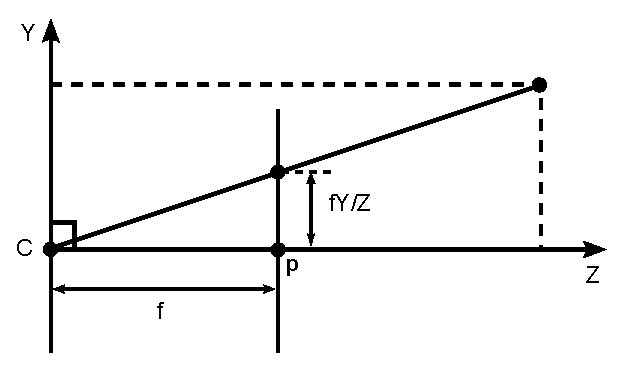
\includegraphics[scale=0.6]{../figs/sizzerman/pinholemodelgeometria}
	  }
	\label{fig:pinholecmaeramodelinterpretation}                %% Etiqueta para la figura entera
	\caption[Modelo de cámara oscura y su interpretación geométrica]{Modelo de cámara oscura \subref{fig:pinholemodel} y su interpretación geométrica \subref{fig:pinholemodel_geometria}. (Figuras adaptadas de \cite{Hartley2004}).}
\end{figure}

Si los puntos son representados mediante una representación homogénea, la proyección central puede expresarse como un mapeo lineal entre coordenadas homogéneas y la notación \eqref{eq:mapeo} puede re-expresarse como en la ecuación \eqref{eq:eq_mapeo_matricial}.
\begin{equation}
\label{eq:eq_mapeo_matricial}
\left(\begin{array}{c}
\mathsf{X}\\
\mathsf{Y}\\
\mathsf{Z}\\
1
\end{array}\right)\mapsto\left(\begin{array}{c}
f\, \mathsf{X}\\
f\, \mathsf{Y}\\
\mathsf{Z}
\end{array}\right)=\left[\begin{array}{cccc}
f & \quad & \quad & 0\\
\quad & f & \quad & 0\\
\quad & \quad & 1 & 0
\end{array}\right]\left(\begin{array}{c}
\mathsf{X}\\
\mathsf{Y}\\
\mathsf{Z}\\
1
\end{array}\right).
\end{equation}

Si se denota con $\mathbf{X}$ al punto de la escena representado por el vector homogéneo $(\mathsf{X},\mathsf{Y},\mathsf{Z},1)^\mathsf{T}$, $\mathbf{x}$ al punto en el plano de la imagen representado por un vector de 3 dimensiones homogéneo y $P$ a la \textit{matriz de proyección de la cámara} homogénea de $3 \times 4$, la expresión \ref{eq:eq_mapeo_matricial} puede ser escrita como
\begin{equation}
 \label{eq:eq_mapeo_matricial_notacion}
  \mathbf{x}=P \mathbf{X}.
\end{equation}

Si bien anteriormente se asumió que el origen de coordenadas en el plano de la imagen se encuentra en el punto principal, en la práctica generalmente esto no es así, por lo que la expresión \ref{eq:mapeo} se puede convertir a una forma más general como se establece en \ref{eq:mapeo_general}, donde $(p_x,p_y)^\mathsf{T}$, son las coordenadas del punto principal. La expresión:
\begin{equation}
  \label{eq:mapeo_general}
  (\mathsf{X},\mathsf{Y},\mathsf{Z})^\mathsf{T} \mapsto (\mathit{f}\mathsf{X}/\mathsf{Z}+p_x, \mathit{f}\mathsf{Y}/\mathsf{Z}+p_y)^\mathsf{T},
\end{equation}
%\ref{eq:mapeo_general}, 
puede ser expresada en coordenadas homogéneas:
%en la ec. \ref{eq:eq_mapeo_matricial_homogeneo}.
\begin{equation}
\label{eq:eq_mapeo_matricial_homogeneo}
\left(\begin{array}{c}
\mathsf{X}\\
\mathsf{Y}\\
\mathsf{Z}\\
1
\end{array}\right)\mapsto\left(\begin{array}{c}
f\, \mathsf{X} + \mathsf{Z}\, p_x\\
f\, \mathsf{Y} + \mathsf{Z}\, p_y\\
\mathsf{Z}
\end{array}\right)=\left[\begin{array}{cccc}
f & \quad & p_x & 0\\
\quad & f & p_y & 0\\
\quad & \quad & 1 & 0
\end{array}\right]\left(\begin{array}{c}
\mathsf{X}\\
\mathsf{Y}\\
\mathsf{Z}\\
1
\end{array}\right).
\end{equation}

Si denotamos con $[I\:|\mathbf{0}]$ la representación de una matriz dividida en un bloque de $3 \times 3$ (la matriz identidad $I$) al que se le concatena un vector columna (un vector de ceros de $[3 \times 1]$ $\mathbf{0}$) y sea la \textit{Matriz de calibración de la cámara}:
\begin{equation}
  \label{eq:k}
  K=\left[\begin{array}{ccc}
	    f & \quad & p_x \\
	    \quad & f & p_y \\
	    \quad & \quad & 1
	  \end{array}\right],
\end{equation}
% definida como en \ref{eq:k}, 
combinando esto en la expresión \ref{eq:eq_mapeo_matricial_homogeneo} se puede llegar a una nueva expresión:
\begin{equation}
\label{eq:mapp_xcam}
\mathbf{x}=K[I\:|\mathbf{0}]\mathbf{X}_{cam},
\end{equation}
donde $\mathbf{X}_{cam}$ %en la ec. \ref{eq:mapp_xcam} 
representa al vector $(\mathsf{X},\mathsf{Y},\mathsf{Z},1)^\mathsf{T}$, asumiéndose que la cámara se encuentra posicionada en el origen del sistema de coordenadas euclídeo con el eje principal de la cámara apuntando en la dirección negativa del eje $\mathsf{Z}$ y donde el punto $\mathbf{X}_{cam}$ está expresado en dicho sistema de coordenadas. Tal sistema de puede denominar como \textit{sistema de coordenadas de la cámara}.

\subsubsection{Parámetros extrínsecos e intrínsecos}
Generalmente los puntos del espacio están expresados en un sistema de coordenadas denominado ``Global''. Este sistema y el \textit{sistema de coordenadas de la cámara} están relacionados mediante una rotación y una traslación como se puede observar en el esquema de la Fig. \ref{fig:transform_between_spaces}. Sea:
\begin{itemize}
 \item $\tilde{\mathbf{X}}$ un vector de 3 dimensiones no homogéneo que representa las coordenadas de un punto en el sistema de coordenadas global,
 \item $\tilde{\mathbf{X}}_{cam}$ el mismo punto, pero en el sistema de coordenadas de la cámara,
 \item $\tilde{\mathbf{C}}$ las coordenadas del centro de la cámara en el sistema global y,
 \item $R$ la matriz de rotación de $3 \times 3$ que representa la orientación del sistema de coordenadas de la cámara,
\end{itemize}
se puede escribir: $\tilde{\mathbf{X}}_{cam}=R(\tilde{\mathbf{X}}-\tilde{\mathbf{C}})$ que en coordenadas homogéneas se puede expresar como:
\begin{equation}
\label{eq:xcam_homogenea}
\mathbf{X}_{cam} = 
\left[\begin{array}{cc}
R & -R \tilde{\mathbf{C}}\\
0 & 1
\end{array}\right]
\left(\begin{array}{c}
\mathsf{X}\\
\mathsf{Y}\\
\mathsf{Z}\\
1
\end{array}\right)
=
\left[\begin{array}{cc}
R & -R \tilde{\mathbf{C}}\\
0 & 1
\end{array}\right]
\mathbf{X}
\end{equation}
y combinado con la expresión \ref{eq:mapp_xcam}, resulta en 
\begin{equation}
\label{eq:xcam_homog_combinado}
\mathbf{x}=KR[I\:|\mathbf{-\tilde{\mathbf{C}}}]\mathbf{X},
\end{equation}
que es la ecuación general de mapeo para el modelo de cámara oscura, donde $\mathbf{X}$ está expresado en coordenadas globales.
\begin{figure}[tbhp]
  \centerline{\includegraphics[scale=0.7]{../figs/sizzerman/transform_between_spaces}}
  \caption[Transformación entre diferentes espacios de coordenadas]{Esquema de transformación euclídea entre el sistema de coordenadas globales y el de la cámara. (Figura adaptada de \cite{Hartley2004}).}
  \label{fig:transform_between_spaces}
\end{figure}
La ecuación \eqref{eq:xcam_homog_combinado} tiene 9 grados de libertad (9DoF): 3 para $K$ $(f,p_x,p_y)$, 3 para $R$ y 3 para $\tilde{\mathbf{C}}$ donde los parámetros de $K$ son conocidos como \textit{parámetros internos de la cámara o intrínsecos} que resultan constantes para un sistema lente-cámara, mientras que los de $R$ y $\tilde{\mathbf{C}}$ son denominados \textit{externos o extrínsecos} y relacionan la orientación de la cámara y la posición del sistema de coordenadas global y resultan ser diferentes para diferentes ``puntos de vista''.

Si no se explicita el centro de la cámara, se puede representar la transformación del sistema global al de la imagen como $\mathbf{\tilde{X}}_{cam}=R \tilde{\mathbf{X}}+\mathbf{t}$ y la matriz de la cámara puede simplificarse a la expresión: %\ref{eq:matrix_camera}
\begin{equation}
 \label{eq:matrix_camera}
P=K[R|\mathbf{t}] \, con \,\,\,\,\, \mathbf{t}=-R \tilde{\mathbf{C}}.
\end{equation}
El modelo de la cámara derivado hasta el momento, asume que las coordenadas de las imagen son coordenadas euclídeas, que tienen igual escala en ambos ejes direccionales. Sin embargo, esto no siempre es así, ya que los píxeles de las cámaras pueden no ser perfectamente cuadrados. Denotando $m_x$  y $m_y$ el número de píxeles por unidad de distancia en las direcciones $x$ e $y$ respectivamente (en coordenadas del plano imagen), se puede obtener una forma general de la matriz de calibración de la cámara mostrada en \ref{eq:k_gral} donde $\alpha_x = fm_x$ y $\alpha_y = fm_y$ representan la distancia focal de la cámara en término de dimensiones de píxeles en la dirección $x$ e $y$ respectivamente, $\mathbf{\tilde{x}}_0=(x_0,y_0)$ es el punto principal con coordenadas $x_0=m_x p_x$ y $y_0 = m_y p_y$ y el parámetro $s$ representa la distorsión de la cámara.
\begin{equation}
  \label{eq:k_gral}
  K=\left[\begin{array}{ccc}
	    \alpha_x & s & x_0 \\
	    \quad & \alpha_y & y_0 \\
	    \quad & \quad & 1
	  \end{array}\right].
\end{equation}
\subsection{Transformación proyectiva y estimación de la homografía}
\label{sec:transf_proyectiva_homograph}
Al tomar dos imágenes de una misma escena desde diferentes puntos de vista, existe una importante relación proyectiva entre éstas y la escena. Estas imágenes, pueden haber sido obtenidas mediante la misma cámara (tomando la fotografía desde dos puntos de vistas diferentes), o mediante dos cámaras posicionadas en diferentes lugares observando el mismo punto.

% La geometría proyectiva 2D es el estudio de las propiedades del plano proyectivo $\mathbb{P}^2$ que son invariantes bajo un grupo de transformaciones proyectivas.
Una transformación proyectiva (también conocida con los términos equivalentes: colineación u homografía) es un mapeo invertible $h$ de $\mathbb{P}^2$ a sí mismo, de tal manera que tres puntos $x_1, x_2, x_3$ están sobre la misma línea si y solo si $h(x_1), h(x_2), h(x_3)$ también lo están. 
\begin{def_transf_proyectiva}
\label{def:transf_proyectiva}
Un mapeo $h$: $\mathbb{P}^2 \rightarrow \mathbb{P}^2$ es
  una transformación proyectiva si y solo si existe una matriz de $3 \times 3$ ($\textit{H}$) tal que para cada punto en $\mathbb{P}^2$ representado por un vector $\mathbf{x}$ se cumple que $h(\mathbf{x})=\textit{H}\mathbf{x}$.
\end{def_transf_proyectiva}
Una definición algebraica se expresa en la Def. \ref{def:transf_proyectiva}, de la que se puede interpretar que:
\begin{itemize}
 \item cualquier punto en $\mathbb{P}^2$ es representado por un vector homogéneo $\mathbf{x}$ de 3 componentes y $\textit{H}\mathbf{x}$ es un mapeo lineal en coordenadas homogéneas,
 \item cualquier transformación lineal invertible de coordenadas homogéneas es una transformación proyectiva.
\end{itemize}
% Una homografía, es un mapeo uno a uno entre dos imágenes que queda definida por ocho parámetros y describe la proyección perspectiva entre dos imágenes tomados desde diferente puntos de vista cuando:
% \begin{itemize}
%   \item El movimiento de la cámara es de rotación pura y 
%   \item La cámara observa una escena plana.
% \end{itemize}
% Si consideramos nuevamente la relación proyectiva existente entre un punto 3D y su imagen en la cámara que se ha introducido en \ref{subsubsection_formacion_imagen}, se ha aprendido que esta relación es expresada por una matriz de $3x4$. Si se considera que las vistas de la escena están separadas puramente mediante una rotación, se puede observar que la cuarta columna de la matriz de parámetros extrínsecos se convierte en 0 (traslación nula). Como resultado, la relación proyectiva en este caso especial da la matriz homografía $H$ de $3x3$. 

Si consideramos el conjunto de puntos $(x_i,y_i,z_i)$ perteneciente a una primer imagen y sabemos que mapean a un conjunto de puntos $(x'_i, y'_i, z'_i)$ en la segunda imagen (ambos en coordenadas homogéneas), la relación entre las dos imágenes es una homografía si se cumple la ecuación %\eqref{eq:eq_cumple_homografia}.
\begin{equation}
  \begin{bmatrix}
  x'_i\\
  y'_i\\
  z'_i
  \end{bmatrix}=\textit{H}
  \begin{bmatrix}
  x_i\\
  y_i \\
  z_i
  \end{bmatrix}\Longrightarrow
\begin{bmatrix}
  x'_i\\
  y'_i\\
  z'_i
  \end{bmatrix}=
  \begin{bmatrix}
  h_{11} & h_{12} & h_{13}\\
  h_{21} & h_{22} & h_{23}\\
  h_{31} & h_{32} & h_{33}\\
  \end{bmatrix}
\begin{bmatrix}
  x_i\\
  y_i \\
  z_i
  \end{bmatrix}.
  \label{eq:eq_cumple_homografia}
\end{equation}

Se puede interpretar de la ecuación \eqref{eq:eq_cumple_homografia} que la homografía $\textit{H}$ mapea coordenadas $x$ en una imagen a coordenadas $x'$ en otra. Es decir, la proyección a través de rayos que pasan a través de un punto en común (el centro de proyección), definen un mapeo de un plano a otro. Este mapeo punto a punto, preserva el mapeo de una línea en un plano a otra línea en otro plano, pero el paralelismo no es necesariamente preservado. Si se considera un plano que pase a través del centro de proyección (Fig. \ref{fig:homografia_esquema}), el mismo intersectaría los planos $\pi$ y $\pi'$ mapeando líneas de un plano a otro. Dado este mapeo, la proyección central es una transformación proyectiva y puede ser representado por un mapeo lineal en coordenadas homogéneas de la forma $\mathbf{x'}=\textit{H}\mathbf{x}$.
\begin{figure}[tbhp]
  \centerline{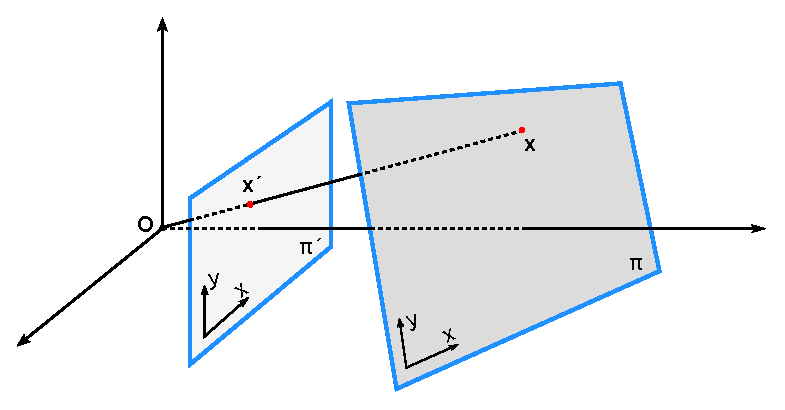
\includegraphics[scale=0.7]{../figs/sizzerman/homografia_esquema}}
  \caption[Mapeo de puntos de un plano a otro]{La proyección central mapea puntos de un plano a puntos en otro plano. (Figura adaptada de \cite{Hartley2004}).}
  \label{fig:homografia_esquema}
\end{figure}
% Si los dos sistemas de coordenadas definidos por los dos planos son sistemas de coordenadas euclídeos (rectilíneos), el mapeo definido por la proyección central es más restrictiva que una transformación proyectiva y recibe el nombre de transformación perspectiva que posee 6 grados de libertad.

La matriz $\textit{H}$ contiene nueve elementos y resulta ambigua al escalarla (el uso de coordenadas homogéneas significa que cualquier múltiplo de la homografía, tendría el mismo efecto). Agregando un factor de escala $s$, la expresión \eqref{eq:eq_cumple_homografia} queda como
\begin{equation}
  \begin{bmatrix} sx'_i \\
  sy'_i\\
  s
  \end{bmatrix}=\textit{H}
  \begin{bmatrix}
  x_i\\
  y_i\\
  1
  \end{bmatrix}.
  \label{eq:eq_ecuacion_rel_homography_ptos}
\end{equation} %\eqref{eq:eq_ecuacion_rel_homography_ptos}. 
Una vez que se a logrado obtener $\textit{H}$, todos los puntos en una vista pueden ser convertidos a la segunda vista usando la relación \ref{eq:eq_ecuacion_rel_homography_ptos}.
% Consecuentemente, como hay solo ocho elementos independientes, se puede obtener la homografía que relaciona dos imágenes usando solo cuatro correspondencias en donde cada correspondencia genera dos ecuaciones lineales.
 %Así, con la transformación proyectiva u homografía \cite{citeulike:9456628, Hartley2004}, se puede aproximar la transformación entre posibles correspondencias de puntos para un par de imágenes.
% Consideremos un conjunto de puntos de correspondencias $x_i \leftrightarrow x'_i$ entre dos imágenes y $P^2$ el plano proyectivo, el problema se reduce a calcular una matriz $H$ de $3x3$ de forma que $Hx_i=x'_i$ para cada $i$. Es decir: dado un conjunto de puntos $x_i \in P^2$ y un conjunto de puntos correspondientes $x'_i \in P^2$, calcular la transformación proyectiva que lleva cada punto $x_i$ a $x'_i$. En una situación práctica $x_i$ e $x_i'$ son puntos en dos imágenes (o la misma) donde cada imagen es considerada como un plano proyectivo $P^2$.
% 
% Para calcular la transformación proyectiva $H$ ser requiere una cantidad de mínima de puntos determinados por el número de grados de libertad y las cantidad de restricciones. Dado que la matriz $H$ contiene 9 valores, en una transformación proyectiva 2D se tienen 8 grados de libertad  (ya que la escala se establece arbitrariamente). Por otro lado, cada correspondencia de puntos involucra dos restricciones, dado que para cada punto $x_i$ en la primer imagen los dos grados de libertad del punto en la segunda imagen deben corresponderse al punto $Hx_i$ mapeado (un punto 2D tiene dos grados de libertad correspondiente a las componentes $x$ e $y$). Alternativamente, el punto es especificado como un vector homogéneo de tres dimensiones que también tiene dos grados de libertad dado que la escala es arbitraria. Como consecuencia, es necesario especificar cuatro correspondencias de puntos con el fin de cumplir la restricción para determinar $H$.

No es común conocer las correspondencias entre puntos de forma exacta, incluso se pueden tener pares de correspondencias que no son válidos o tener más de 4 pares de correspondencias en cuyo caso la matriz $\textit{H}$ puede resultar incorrecta. Por ello, para estos casos, se procede mediante una \textit{estimación} de la homografía.
% . Sea $\mathbf{X}$ un punto en la superficie plana con proyecciones $\mathbf{x}_i$ y $\mathbf{x'}_i$, en dos imágenes tomadas desde diferentes puntos de vista, la Homografía $H$, describe la transformación que conecta $\mathbf{x}_i$ y $\mathbf{x'}_i$ para cualquier punto $\mathbf{X}$ en la superficie, esto es $\mathbf{x'}_i=H\mathbf{x}_i$. 

% La misma es buscada de tal forma que el error de retro-proyección sea minimizado. Usualmente todos los pares son usados para buscar la homografía, sin embargo las coincidencias comúnmente tiene valores espurios que mediante 
\subsubsection{Estimación de la homografía}
\label{sec:estimacion_ransac_homografia}
Si se conocen exactamente cuatro correspondencias (tres de ellas no colineales), se puede encontrar una solución exacta de la matriz $\textit{H}$. Esta solución es denominada ``solución mínima'' y resulta importante ya que define el subconjunto mínimo requerido para los algoritmos de estimación robusta como RANSAC. En la práctica, generalmente se conocen más de cuatro correspondencias (válidas o no) y estas correspondencias no resultan totalmente compatibles con una transformación proyectiva. Por ello, nos encontramos con la tarea de determinar la ``mejor'' transformación a partir de los datos, lo cual se convierte en la búsqueda de la transformación $\textit{H}$ que minimice una función de costo.
% Usualmente hay una función de costo que resulta óptima en el sentido de que la $H$ que minimiza, da la mejor estimación posible de la transformación bajo ciertos supuestos. En el caso de la estimación de la homografía entre dos vistas es el error de reproyección.
\paragraph{Transformación lineal directa.} 
La transformación lineal directa o DLT (del inglés, Direct Linear Transform) es un algoritmo lineal para determinar $\textit{H}$ dado un conjunto de 4 puntos 2D correspondientes $\mathbf{x_{\textrm{i}}\leftrightarrow x_{\textrm{i}}^{\textrm{\ensuremath{\prime}}}}$. La transformación viene dada por la ecuación 
$\mathbf{x_{\textrm{i}}^{\textrm{\ensuremath{\prime}}}=\textrm{\textit{H}}x_{\textrm{i}}}$ donde los vectores están dados en coordenadas homogéneas, es decir que $\mathbf{x_{\textrm{i}}^{\textrm{\ensuremath{\prime}}}}$ y $\mathbf{\textrm{\textit{H}}x_{\textrm{i}}}$  no son iguales (tienen la misma dirección pero pueden diferir en magnitud por un escalar que no sea cero). Denotando $\mathbf{x_{\textrm{i}}=}(x_{i},y_{i},w_{i})^{\mathsf{T}}$, $\mathbf{x_{\textrm{i}}^{\prime}=}(x_{i}^{\prime},y_{i}^{\prime},w_{i}^{\prime})^{\mathsf{T}}$ y $\textit{H}=\left(\begin{array}{c}
\mathbf{\mathbf{h^{\textrm{1}\mathsf{T}}}}\\
\mathbf{h}^{\textrm{2}\textsf{T}}\\
\mathbf{h}^{\textrm{3}\textsf{T}}
\end{array}\right)$, donde $\mathbf{h^{\textrm{i}\textsf{T}}}$ es un vector fila que denota la fila $i$ de $\textit{H}$, mediante algunos cálculos \cite[p. 89]{Hartley2004} y teniendo presente que el sistema $\mathbf{x_{\textrm{i}}^{\textrm{\ensuremath{\prime}}}=\textrm{\textit{H}}x_{\textrm{i}}}$ posee tres ecuaciones, de las cuales solo dos son independientes (la tercera fila es obtenida para un factor de escala) %de la suma de de $x_{i}^{\prime}$ veces la primera fila y $y_{i}^{\prime}$ veces la segunda) 
se obtiene
\begin{equation}
\begin{bmatrix}\mathbf{0}^{\textsf{T}} & -w_{i}^{\prime}\mathbf{x_{\textrm{i}}^{\textrm{\textsf{T}}}} & y_{i}^{\prime}\mathbf{x_{\textrm{i}}^{\textrm{\textsf{T}}}}\\
w_{i}^{\prime}\mathbf{x_{\textrm{i}}^{\textrm{\textsf{T}}}} & \mathbf{0}^{\textsf{T}} & -x_{i}^{\prime}\mathbf{x_{\textrm{i}}^{\textrm{\textsf{T}}}}
\end{bmatrix}\begin{pmatrix}\mathbf{h^{\textrm{1}}}\\
\mathbf{h^{\textrm{2}}}\\
\mathbf{h^{\textrm{3}}}
\end{pmatrix}=\mathbf{0}.\label{eq:hxsystem}
\end{equation}

El sistema \ref{eq:hxsystem} se puede escribir como $A_{i} \mathbf{h}=\mathbf{0}$ donde $A_{i}$ es la matriz de $2 \times 9$ y $\mathbf{h}$ el vector de $9 \times 1$ de la ecuación \eqref{eq:hxsystem}. Para cada correspondencia de puntos se obtienen 2 ecuaciones, por lo que 4 correspondencias (forman un sistema de $8 \times 8$) resultan suficientes para resolver los 8 grados de libertad de $\textit{H}$ (recordar que se determina para un factor de escala), siempre que se tengan al menos 3 puntos no colineales.
% Este conjunto de cuatro correspondencias, se obtiene un conjunto de ecuaciones $A\mathbf{h}=\mathbf{0}$, donde $A$ es una matriz cuyos coeficientes son los que resultan de las filas de la matriz $A_{i}$ que da cada correspondencia y $\mathbf{h}$ es el vector de los coeficientes de $H$ que se debe determinar (se busca la solución que no sea $\mathbf{h}=\mathbf{0}$, ya que esta resulta de interés).

Si se tienen más de cuatro correspondencias $\mathbf{x_{\textrm{i}}\leftrightarrow x_{\textrm{i}}^{\textrm{\ensuremath{\prime}}}}$, el conjunto de ecuaciones $A\mathbf{h}=\mathbf{0}$ tiene muchas soluciones. Además, si estas correspondencias no son exactas, la solución encontrada no será adecuada, por lo que el problema se convierte en estimar la homografía minimizando una función de error \cite{Hartley2004}.

Existen algoritmos como \textit{least median of squares} (LMEDS) \cite{Rousseuw_1994} o el de \textit{random sample consensus} (RANSAC)\cite{Fischler:1981:RSC:358669.358692, Hartley2004} que pueden hallar la mejor solución aproximada minimizando el error y a su vez, tratando de detectar cuáles son los supuestos valores de coincidencias válidos (del inglés, inliers) y los espurios (del inglés, outliers). Además son capaces de utilizar más de cuatro correspondencias para obtener una solución más exacta. El método LMEDS, a diferencia del RANSAC, no necesita un umbral para distinguir entre las correspondencias válidas y las espurias, sin embargo, LMEDS sólo funciona correctamente cuando hay más de un $50\%$ de valores válidos \cite{Hartley2004, BenhimaneNGGNM08}.
\paragraph{Homografía con RANSAC.}
El objetivo que se plantea aquí, es el de determinar un conjunto de correspondencias (eliminando valores espurios) de forma que la homografía pueda ser estimada de manera óptima a partir de las mismas mediante la transformación lineal directa descripta.

Para explicar y entender el algoritmo RANSAC, primero se presenta un problema que puede ser fácilmente visualizado el cual consiste en estimar una línea recta a partir de un conjunto de puntos 2D. Este problema, también puede pensarse sobre como realizar la estimación de una transformación afín 1D del tipo $x'=ax+b$ entre puntos correspondientes que están sobre dos líneas. 

El problema, se encuentra ilustrado en la Fig. \ref{fig:example_ransac}(a) (los puntos negros son válidos y los blancos son espurios) donde se puede ver que el ajuste por mínimos cuadrados de los puntos (regresión ortogonal), es afectado de forma severa por los valores espurios. Así, dado un conjunto de puntos 2D, se debe buscar la línea que minimiza la suma de los cuadrados de las distancias perpendiculares, %(regresión ortogonal), 
de tal forma que ninguno de los puntos válidos se desvíe de la línea por más de $t$ unidades. Aquí, se presentan dos inconvenientes: la línea se debe ajustar a los datos y se deben clasificar los puntos en válidos o espurios.

Existen muchos tipos de algoritmos robustos y la selección de uno u otro depende de la proporción de los valores espurios \cite{Hartley2004}. Aquí se describe el estimador robusto RANSAC que es capaz de hacer frente a una gran proporción de valores atípicos.

Se empieza mediante la selección aleatoria de dos puntos; estos puntos definen una línea. El \textit{soporte} para esta línea, es medido por la cantidad de puntos que se encuentran bajo un umbral de distancia. Luego, la selección aleatoria es repetida varias veces y la línea con mayor soporte es considerada como el mejor ajuste. Los puntos que están por debajo del umbral de distancia son considerados válidos y constituyen el \textit{conjunto consensuado}. Como se observa en la Fig. \ref{fig:example_ransac}(b), si un punto no es válido, la línea posee menos soporte lo cual favorece a un mejor ajuste. Por ejemplo, el soporte para la línea $<\mathbf{a},\mathbf{b}>$ en la Fig. \ref{fig:example_ransac}(b) es 10, mientras que para la línea $<\mathbf{a},\mathbf{d}>$ en el que los puntos de ejemplo son vecinos, es 4. Consecuentemente y a pesar que ambas líneas contienen valores válidos, se selecciona la línea $<\mathbf{a},\mathbf{b}>$ por tener mayor soporte.
\begin{figure}[tbhp]
  \centerline{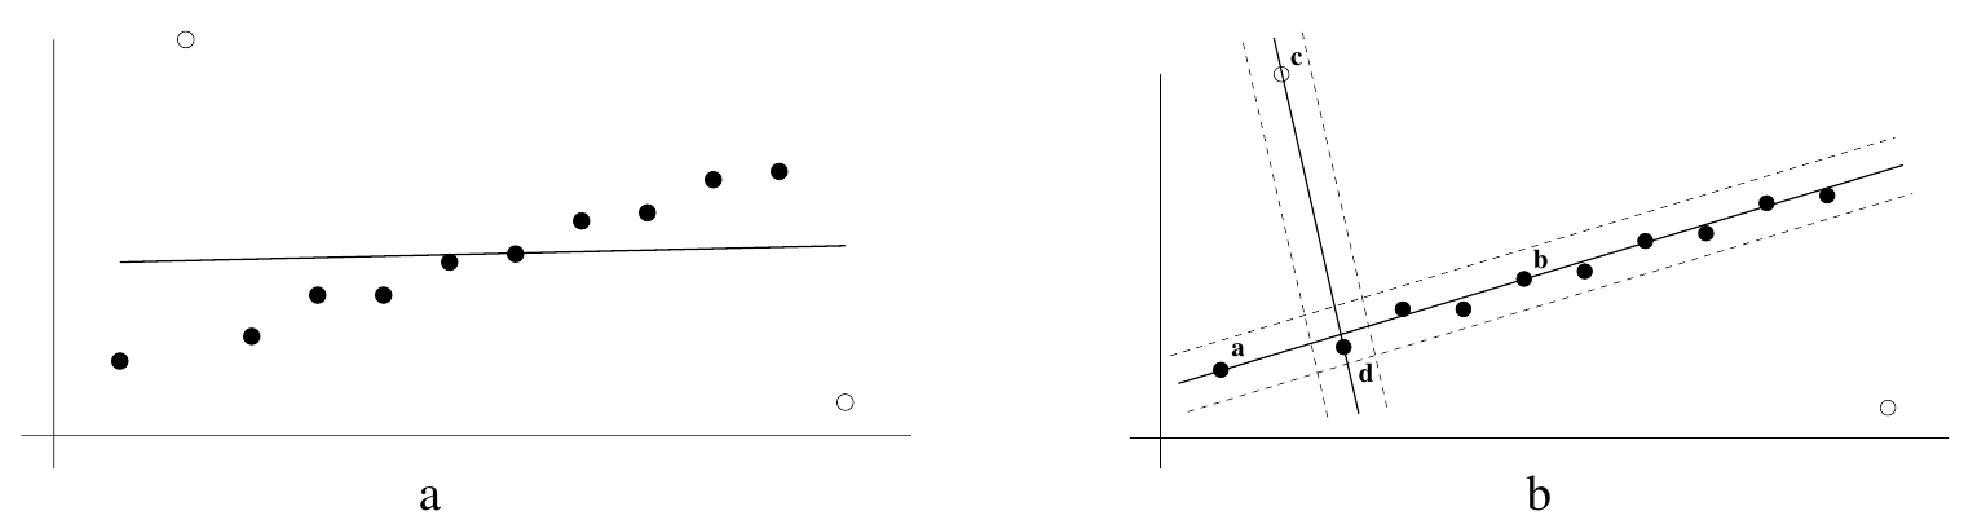
\includegraphics[scale=0.4]{../figs/robust_line_estimation}}
  \caption[Estimación robusta de una línea]{Estimación robusta de una línea. (a) Ajuste por mínimos cuadrados. (b) Algoritmo RANSAC (las líneas punteadas denotan el umbral de distancia). (Figura tomada de \cite{Hartley2004}).}
\label{fig:example_ransac}  
\end{figure}

Generalizando lo anteriormente descripto, podemos decir que deseamos ajustar un \textit{modelo} (en el ejemplo, una línea) a los datos y la muestra aleatoria consiste en un subconjunto mínimo de datos (2 puntos en el ejemplo) suficientes para determinar el modelo. En el caso en el que el modelo es una homografía plana y los datos son un conjunto de correspondencias 2D, el subconjunto mínimo está compuesto por cuatro correspondencias.

El algoritmo RANSAC tiene como objetivo el ajuste robusto de un modelo para un conjunto de datos $S$ que contiene valores espurios. RANSAC requiere de una cantidad mínima de puntos $s$ para instanciar los parámetros libres del modelo y sigue los siguientes pasos:

\fcolorbox{black}[HTML]{EDEDED}{\parbox{365pt}{%
\noindent %\textbf{Eksempel.}
\begin{enumerate}[nolistsep]
 \item Se seleccionan aleatoriamente un conjunto de puntos $s \in S$ y se instancia el modelo para este subconjunto,
 \item Se determina el conjunto de puntos $S_i$ que se encuentran dentro de un umbral de distancia $t$ respecto al modelo. El conjunto $S_i$ es el conjunto consensuado de muestras y define los valores válidos de $S$.
 \item Si la cantidad de elementos válidos en $S_i$ es mayor que un umbral $T$, se estima nuevamente el modelo usando todos los puntos de $S_i$ y se termina el algoritmo.
 \item Si la cantidad de elementos válidos en $S_i$ es menor que $T$, se selecciona un nuevo subconjunto y se repiten los pasos arriba mencionados.
 \item Luego de $N$ iteraciones, el conjunto consensuado $S_i$ con mayor cantidad de elementos es seleccionado y se estima el modelo usando este conjunto de datos.
\end{enumerate}}}

donde $t$, $N$ y $T$ son:
\begin{itemize}
  \item \textbf{Umbral de distancia $t$:} Existen diferentes medidas de distancias, como la de transferencia del error simétrico, la del error de Sampson y la del error de reproyección que resulta la más adecuada en el caso de la estimación de la homografía entre dos imágenes \cite{Hartley2004}. La fórmula del error de reproyección, viene dada por la ecuación ${d_{\perp}}^{2}=d(\mathbf{x},\mathbf{\hat{x}})^2+d(\mathbf{x^\prime},\mathbf{\hat{x}^\prime})^2$ donde $\mathbf{x} \leftrightarrow \mathbf{x^\prime}$ es la correspondencia de puntos y $\mathbf{\hat{x}^\prime}=\textit{H}\mathbf{\hat{x}}$ es la correspondencia exacta. Aquellos puntos que cumplan la condición ${d_{\perp}}^{2}>t^2$ son considerados como espurios y los que cumplan con ${d_{\perp}}^{2} \leq t^2$ son considerados válidos. Es usual que en la práctica el valor de $t$ sea seleccionado empíricamente, sin embargo si se asume que la medida del error tiene una distribución gaussiana con media 0 y desviación estándar $\sigma$ puede calcularse el valor de $t$. Por ejemplo, para el caso de la homografía, con una una probabilidad del $95\%$ de que la correspondencia sea válida se utiliza $t^2=5.99\sigma^2$. Para más destalles se puede consultar \cite[p. 119]{Hartley2004}.
  \item \textbf{Tamaño del Conjunto consensuado $T$:} la regla es terminar el algoritmo si el tamaño del conjunto consensuado es similar a la cantidad de valores válidos que se cree que está presente en el conjunto de datos, dada la premisa de la proporción de valores espurios que, por ejemplo, para $n$ puntos es $T=(1-\epsilon)n$.
  \item \textbf{Cantidad de muestras $N$:} es computacionalmente innecesario e ineficiente probar cada muestra posible. Por eso, se selecciona una cantidad de muestras $N$ lo suficientemente alta para asegurar con una probabilidad $p$, que por lo menos una de las muestras aleatorias de $s$ puntos, no contiene puntos espurios. Usualmente se establece a $p=0.99$ \cite{Hartley2004}. Si suponemos que $w$ es la probabilidad que cualquier punto seleccionado de los datos es un punto válido, implica que $\epsilon=1-w$ representa la probabilidad que sea un punto espurio. Luego, se necesitan $N$ selecciones, cada una de $s$ puntos, donde $(1-w^s)^{N}=1-p$. Así, $N$ queda definida como:
  \begin{equation}
    N=\log(1-p)/\log{(1-(1-\epsilon)^s)}.
    \label{eq:determineN}
  \end{equation}

Para $s=4$ muestras, con una proporción de valores espurios del $\epsilon=50\%$, son necesarias 72 muestras para asegurarse con una probabilidad de $p=0.99$, que al menos una de las muestras no contiene valores espurios. Como se observa en la ecuación \eqref{eq:determineN}, la cantidad de muestras está relacionada con la proporción de valores espurios, de forma que la cantidad de muestras requeridas debe ser menor que la cantidad de valores espurios. Consecuentemente, el costo computacional de las muestras es aceptable aún cuando la cantidad de valores espurios resulta elevado. Por otro lado, la cantidad de muestras se incrementa con la cantidad mínima del subconjunto (para un $\epsilon$ y $p$ dado). De aquí, se puede decir que usar más del mínimo que se requiere (4 o más puntos en el caso de la homografía), contribuirá a una mejor estimación y el soporte determinado reflejará con mayor precisión al verdadero soporte. Pero se debe tener en cuenta que esta ventaja, incrementa el costo computacional debido al incremento del número de muestras.
\end{itemize}
% En lo que respecta a la selección de muestras, se debe tener en cuenta que las muestras ``degeneradas'' deben ser tenidas en cuenta. Por ejemplo, cuando de los cuatro puntos se tienen tres puntos que son colineales, la homografía no puede calcularse.%; además, las muestras deben consistir en puntos con una buena distribución espacial sobre la imagen.
% %%
\subparagraph{Determinación adaptativa de la cantidad de muestras}
Por lo general $\epsilon$ es desconocido por lo que en dicho caso, el algoritmo es inicializado usando el peor caso de estimación de $\epsilon$, y esta estimación es actualizada a medida que se encuentran más conjuntos consistentes. Por ejemplo, si se supone que el peor caso es $\epsilon=0.5$ y del conjunto consensuado se encuentra un $80\%$ de datos como válidos, la estimación actualizada es $\epsilon=0.2$.

La idea de ``probar'' los datos mediante el conjunto consensuado puede ser aplicada repetidamente para de determinar adaptativamente la cantidad de muestras $N$. Si tenemos en cuenta el ejemplo mencionado en el párrafo anterior, la peor estimación $\epsilon=0.5$ determina el valor inicial de $N$ en base a la ecuación \eqref{eq:determineN}. Cuando el conjunto consensuado contiene más del $50\%$ de datos encontrados, sabemos que hay por lo menos esa misma cantidad de valores válidos. Esta estimación actualizada de $\epsilon$ determina un $N$ reducido de acuerdo a la ecuación \eqref{eq:determineN}. Esta actualización es repetida para cada muestra y cada vez que es encontrado un conjunto consensuado con $\epsilon$ menor que el ya estimado, la cantidad $N$ también disminuye. El algoritmo termina tan pronto como $N$ muestras han sido analizadas.

Los pasos que se siguen para la determinación adaptativa de la cantidad de muestras como así también la proporción de valores espurios de cada conjunto consensuado, son los siguientes:

\fcolorbox{black}[HTML]{EDEDED}{\parbox{365pt}{%
\noindent %\textbf{Eksempel.}
\begin{enumerate}[nolistsep]
 \item $N=\infty$, $contador\_muestras=0$.
 \item Mientras $N>contador\_muestras$ repetir:
  \begin{itemize}
    \item Seleccionar una muestra y contar el número de valores válidos. 
    \item Establecer $\epsilon=1-\frac{\text{cantidad de valores válidos}}{\text{cantidad total de puntos}}$
    \item Establecer $N$ con $\epsilon$ según la ecuación \eqref{eq:determineN} para $p=0.99$
    \item Incrementar $contador\_muestras$ por 1
  \end{itemize}
 \item Fin.
\end{enumerate}}}

\smallskip
El algoritmo RANSAC, es aplicado a las potenciales correspondencias para estimar la homografía como así también las correspondencias válidas consistentes con dicha estimación. Como se ha mencionado, cuatro correspondencias son suficientes para determinar la homografía (siempre que no hayan tres colineales), sin embargo, se puede obtener una mejor estimación usando todos los valores válidos (en vez de sólo cuatro), además de obtener un conjunto con mayor cantidad de correspondencias válidas de forma que la homografía resulte más precisa. Esto, se logra con la minimización de la función del error de reproyección mediante el algoritmo Levenberg-Marquardt (método iterativo con una variación al método iterativo de Gauss-Newton \cite[p. 600]{Hartley2004}). Todos los pasos descriptos para la estimación de la homografía se describen a continuación:

\fcolorbox{black}[HTML]{EDEDED}{\parbox{365pt}{%
\noindent \textbf{Cálculo de la homografía 2D entre dos imágenes.}
\begin{enumerate}[nolistsep]
 \item Se asume que se tiene un conjunto de potenciales correspondencias entre las imágenes.
 \item Se repite para $N$ muestras ($N$ determinado con el algoritmo adaptativo)
  \begin{itemize}
    \item Se seleccionan aleatoriamente cuatro correspondencias y se calcula la homografía $\textit{H}$.
    \item Se calcula la distancia $d_{\perp}$ para cada correspondencia.
    \item Se calcula la cantidad de valores válidos consistentes con $\textit{H}$ entre la cantidad de correspondencias para las cuales $d_{\perp}<t=\sqrt{5.99}\sigma$ píxeles.
  \end{itemize}
  Seleccionar $\textit{H}$ con la mayor cantidad de valores válidos. 
 \item Re-estimar $\textit{H}$ a partir de todas las correspondencias clasificadas como válidas, mediante la minimización de la función acumulada de error de reproyección: $\underset{i}{\sum}d(\mathbf{x}_{i},\hat{\mathbf{x}}_{i})^{2}+d(\mathbf{x}_{i}^{\prime},\hat{\mathbf{x}}_{i}^{\prime})^{2}$ sujeto a $\hat{\mathbf{x}}_{i}^\prime=\hat{\textit{H}}\hat{\mathbf{x}_i}\; \forall i$ usando el algoritmo de Levenberg-Marquardt.
\end{enumerate}}}